%%% Exemplo de utilização da classe ITA
%%%
%%%   por        Fábio Fagundes Silveira   -  ffs [at] ita [dot] br
%%%              Benedito C. O. Maciel     -  bcmaciel [at] ita [dot] br
%%%              Giovani Volnei Meinertz   -  giovani [at] ita [dot] br
%%%    	         Hudson Alberto Bode       -  bode [at] ita [dot]br
%%%    	         P. I. Braga de Queiroz    -  pi [at] ita [dot] br
%%%    	         Jorge A. B. Gripp         -  gripp [at] ita [dot] br
%%%    	         Juliano Monte-Mor         -  jamontemor [at] yahoo [dot] com [dot] br
%%%    	         Tarcisio A. B. Gripp      -  tarcisio.gripp [at] gmail [dot] com
%%%
%%%   Versão para overleaf:
%%%   por        Alejandro A. Rios Cruz    - aarc.88@gmail.com
%%%              Saulo Gómez               - sagomezs@unal.edu.co
%%%              Ocimar Santos             - ocimar.acad@gmail.com
%%%
%%%   Template disponibilizado em:
%%%              Overleaf: https://pt.overleaf.com/latex/templates/thesis-template-aeronautics-institute-of-technology-ita/yhfrqqydpygk
%%%
%%%   Contribuia você também!
%%%              GitHub:   https://github.com/gabriellnuness/Template_Thesis_ITA
%%%
%%%  IMPORTANTE: O texto contido neste exemplo nao significa absolutamente nada.  :-)
%%%              O intuito aqui eh demonstrar os comandos criados na classe e suas
%%%              respectivas utilizacoes.
%%%
%%%  Tese.tex  2016-08-25
%%%  $HeadURL: http://www.apgita.org.br/apgita/teses-e-latex.php $
%%%
%%% ITALUS
%%% Instituto Tecnológico de Aeronáutica --- ITA, Sao Jose dos Campos, Brasil
%%%                   http://groups.yahoo.com/group/italus/
%%% Discussion list: italus {at} yahoogroups.com
%%%
%++++++++++++++++++++++++++++++++++++++++++++++++++++++++++++++++++++++++++++++
% Para alterar o TIPO DE DOCUMENTO, preencher a linha abaixo \documentclass[?]{?}
%   \documentclass[tg]{ita}			= Trabalho de Graduacao
%   \documentclass[tgfem]{ita}	= Para Engenheiras
%   								msc     		= Dissertacao de Mestrado
%   								mscfem   		= Para Mestras
%   								dsc      		= Tese de Doutorado
%   								dscfem   		= Para Doutoras
%   								quali    		= Exame de Qualificacao
%   								qualifem 		= Exame de Qualificacao para Doutoras
% Para 'Draft Version'/'Versao Preliminar' com data no rodape, adicionar 'dv':
%   \documentclass[dsc, dv]{ita}
% Para trabalhos em Inglês, adicionar 'eng':
%   \documentclass[dsc, eng]{ita}
%		\documentclass[dsc, eng, dv]{ita}
%++++++++++++++++++++++++++++++++++++++++++++++++++++++++++++++++++++++++++++++
\documentclass[tg, eng]{ita}    % ITA.cls based on standard book.cls
% Quando alterar a classe, por exemplo de [msc] para [msc, eng]) rode mais uma vez o botão BUILD OUTPUT caso haja erro
\usepackage{ae}
\usepackage{graphicx}
\usepackage{epsfig}
\usepackage{amsmath}
\usepackage{amssymb}
\usepackage{subfig}
\usepackage{multirow}
\usepackage{float}
\usepackage{amsthm}
\usepackage{url}         % formats URL addresses properly
\usepackage{appendix}    % allows appendix section to be included
\usepackage{lscape}      % allows a page to be rendered in landscape mode
\usepackage{multicol}    % allows text in multi columns
\usepackage{cancel}      % needed to show canceled terms in equations
\usepackage{lettrine}
\usepackage{float}
\usepackage{placeins}


%HHHHHHHHHHHHHHHHHHHHHHHHHHHHHHHHHHHHHHHHHHHHHHHHHHHHHHHHHHHHHHHHHHHHHHHHHHHHHHHHHHHHHHHHHHHHHHHHHHHHHHHHHHHH
\addbibresource{Referencias/referencias.bib}

%HHHHHHHHHHHHHHHHHHHHHHHHHHHHHHHHHHHHHHHHHHHHHHHHHHHHHHHHHHHHHHHHHHHHHHHHHHHHHHHHHHHHHHHHHHHHHHHHHHHHHHHHHHHH
%\usepackage{subfigure}
%\usepackage{subfigmat}
%PACOTEFIGURAS_SE _ERRADO_ESXCLUIR_ACIMA
\usepackage{booktabs}
\usepackage{threeparttable}
\usepackage[table]{xcolor}
%PACOTETABELAS_SE _ERRADO_ESXCLUIR_ACIMA
\usepackage{tikz}
\usetikzlibrary{arrows.meta,shapes,positioning}
\usepackage{tkz-euclide}
%HHHHHHHHHHHHHHHHHHHHHHHHHHHHHHHHHHHHHHHHHHHHHHHHHHHHHHHHHHHHHHHHHHHHHHHHHHHHHHHHHHHHHHHHHHHHHHHHHHHHHHHHHHHH

%++++++++++++++++++++++++++++++++++++++++++++++++++++++++++++++++++++++++++++++
% Espaçamento padrão de todo o documento
%++++++++++++++++++++++++++++++++++++++++++++++++++++++++++++++++++++++++++++++
\onehalfspacing

%singlespacing Para um espaçamento simples
%onehalfspacing Para um espaçamento de 1,5
%doublespacing Para um espaçamento duplo

%++++++++++++++++++++++++++++++++++++++++++++++++++++++++++++++++++++++++++++++
% Identificacoes (se o trabalho for em inglês, insira os dados em inglês)
% Para entradas abreviadas de Professora (Profa.) em português escreva: Prof$^\textnormal{a}$.
%++++++++++++++++++++++++++++++++++++++++++++++++++++++++++++++++++++++++++++++
\course{Electronic Engineering}  % Programa de PG ou Curso de Graduacao
\area{} % Área de concentração na PG (Não utilizado no caso de TG)

% Autor do trabalho: Nome Sobrenome
\authorgender{masc}                     %sexo: masc ou fem
\author{Mario Célio}{da Silva Bezerra}
\itaauthoraddress{Rua H8B, Ap. 241}{12.228-461}{São José dos Campos--SP}

% Titulo da Tese/Dissertação
\title{
% \color{red}
A Vectorized Reinforcement Learning Framework for IEEE Very Small Size Soccer
}


% Orientador
\advisorgender{masc}                    % masc ou fem
\advisor{Prof.~Dr.}{Marcos Máximo}{ITA}

% Coorientador (Caso não haja coorientador, colocar ambas as variáveis \coadvisorgender e \coadvisor comentadas, com um % na frente)
% \coadvisorgender{fem}									% masc ou fem
% \coadvisor{Prof$^\textnormal{a}$.~Dr$^\textnormal{a}$.}{Doralice Serra}{OVNI}

% TODO: remove Pro-rector entry or just leave it optional and off by default?
% Pró-reitor da Pós-graduação
% \bossgender{masc}												% masc ou fem
% \boss{Prof.~Dr.}{John von Neumann}

%Coordenador do curso no caso de TG
\bosscoursegender{masc}									% masc ou fem
\bosscourse{Prof.~Dr.}{Marcelo Pinho}

% Palavras-Chaves informadas pela Biblioteca -> utilizada na CIP
\kwcip{Reinforcement Learning}
\kwcip{Multi-Agent Systems}
\kwcip{VSSS}
\kwcip{GPU Simulation}

% membros da banca examinadora

\examiner{Prof. Dr.}{Marcos Máximo}{Advisor}{ITA}
\examiner{Prof. Dr.}{José Roberto Colombo}{Electronic Engineering Department}{ITA}
\examiner{Master's Student}{Kenji Yamane}{T23}{ITA}
% \examiner{Prof. Dr.}{Examiner Name}{}{Institution}

% Data da defesa (mês em maiúsculo, se trabalho em inglês, e minúsculo se trabalho em português)
\date{29}{May}{2026}

% Número CDU - (somente para TG)
\color{red}
\cdu{???.???}
\color{black}
% Glossario
\makenoidxglossaries % to use glossaries pkg
\frontmatter


%%%%%%%% acronyms %%%%%%%%
\newacronym{api}{API}{Application Programming Interface}
\newacronym{cpu}{CPU}{Central Processing Unit}
\newacronym{ctde}{CTDE}{Centralized Training with Decentralized Execution}
\newacronym{drl}{DRL}{Deep Reinforcement Learning}
\newacronym{gae}{GAE}{Generalized Advantage Estimation}
\newacronym{gpu}{GPU}{Graphics Processing Unit}
\newacronym{jax}{JAX}{Just After eXecution}
\newacronym{jit}{JIT}{just-in-time compilation}
\newacronym{marl}{MARL}{Multi-Agent Reinforcement Learning}
\newacronym{mlp}{MLP}{Multilayer Perceptron}
\newacronym{mdp}{MDP}{Markov Decision Process}
\newacronym{ode}{ODE}{Open Dynamics Engine}
\newacronym{ogre}{OGRE}{Object-Oriented Graphics Rendering Engine}
\newacronym{plr}{PLR}{Prioritized Level Replay}
\newacronym{ppo}{PPO}{Proximal Policy Optimization}
\newacronym{rl}{RL}{Reinforcement Learning}
\newacronym{trpo}{TRPO}{Trust Region Policy Optimization}
\newacronym{vsss}{VSSS}{Very Small Size Soccer}

\newglossaryentry{discount_factor}{name=\ensuremath{\gamma}, description={Discount factor}, sort={gamma}}

\newglossaryentry{policy}{name=\ensuremath{\pi_\theta}, description={Policy parameterized by $\theta$}, sort={pi_theta}}

\newglossaryentry{state_space}{name=\ensuremath{\mathcal{S}}, description={State space}, sort={S}}

\newglossaryentry{action_space}{name=\ensuremath{\mathcal{A}}, description={Action space}, sort={A}}

\newglossaryentry{value_function}{name=\ensuremath{V^\pi(s)}, description={State-value function under policy $\pi$}, sort={V}}

\newglossaryentry{advantage_function}{name=\ensuremath{A^\pi(s,a)}, description={Advantage function under policy $\pi$}, sort={A_adv}}

\newglossaryentry{linear_velocity}{name=\ensuremath{v}, description={Robot linear velocity}, sort={v}}

\newglossaryentry{angular_velocity}{name=\ensuremath{\omega}, description={Robot angular velocity}, sort={omega}}

\newglossaryentry{wheel_base}{name=\ensuremath{L}, description={Distance between wheel contact points (wheelbase)}, sort={L}}

\newglossaryentry{wheel_diameter}{name=\ensuremath{d}, description={Wheel diameter}, sort={d}}

\newglossaryentry{wheel_speed_left}{name=\ensuremath{\omega_l}, description={Left wheel angular velocity}, sort={omega_l}}

\newglossaryentry{wheel_speed_right}{name=\ensuremath{\omega_r}, description={Right wheel angular velocity}, sort={omega_r}}

\newglossaryentry{control_freq}{name=\ensuremath{f_c}, description={Simulator control frequency}, sort={f_c}}

\newglossaryentry{num_substeps}{name=\ensuremath{N_{\mathrm{sub}}}, description={Number of physics sub-steps per control step}, sort={N_sub}}

\newglossaryentry{max_speed}{name=\ensuremath{v_{\max}}, description={Maximum robot linear speed}, sort={v_max}}

\newglossaryentry{slew_limit}{name=\ensuremath{a_{\mathrm{slew}}}, description={Wheel angular acceleration limit (slew rate)}, sort={a_slew}}

\newglossaryentry{shaping_coef}{name=\ensuremath{\beta}, description={Forward ball progress shaping coefficient}, sort={beta}}

\newglossaryentry{crowd_penalty_coeff}{name=\ensuremath{\lambda_c}, description={Foul Play penalty coefficient}, sort={lambda_c}}

\newglossaryentry{pos_x}{name=\ensuremath{x}, description={Position x-coordinate (field frame)}, sort={x}}

\newglossaryentry{pos_y}{name=\ensuremath{y}, description={Position y-coordinate (field frame)}, sort={y}}

\newglossaryentry{vel_x}{name=\ensuremath{v_x}, description={Linear velocity x-component}, sort={v_x}}

\newglossaryentry{vel_y}{name=\ensuremath{v_y}, description={Linear velocity y-component}, sort={v_y}}

\newglossaryentry{heading}{name=\ensuremath{\theta}, description={Robot heading angle}, sort={theta}}

\newglossaryentry{friction_coef}{name=\ensuremath{\mu_r}, description={Ball rolling friction coefficient}, sort={mu_r}}

\newglossaryentry{foul_penalty_coeff}{name=\ensuremath{\gamma_{\mathrm{foul}}}, description={Foul Play penalty coefficient}, sort={gamma_crowd}}

\begin{document}
% Folha de Rosto e Capa para o caso do TG
\maketitle

% Dedicatoria: Nao esqueca essa secao  ... :-)
% \begin{itadedication}
% \color{red}
% dedicatoria to-be written
% \end{itadedication}

% Agradecimentos
% \begin{itathanks}
% \color{red}
I thank my advisor, Prof.~Dr. Marcos Máximo, for the guidance and support during the development of this work.

I also thank the ITAndroids team for the motivation to this project.

% \end{itathanks}

% Epígrafe
% \ifhyperref\pdfbookmark[0]{\nameepigraphe}{epigrafe}\fi
% \begin{flushright}
% \begin{spacing}{1}
% \mbox{}\vfill
% {\color{red}
{\sffamily\itshape
``If I have seen farther than others,\\
it is because I stood on the shoulders of giants.''\\}
--- \textsc{Sir~Isaac Newton}}

% \end{spacing}
% \end{flushright}

% Resumo
\begin{abstract}
\noindent
Este trabalho aborda o treinamento por aprendizado por reforço em larga escala no futebol de robôs IEEE Very Small Size Soccer em partidas 3v3 por meio de duas contribuições: um simulador em GPU baseado em JAX, capaz de executar milhares de partidas em paralelo, e uma pipeline de treinamento PPO para uma política centralizada de equipe. O throughput de treinamento PPO de ponta a ponta alcança aproximadamente $49{.}000$--$58{.}000$ passos por segundo (com 256 e 65{.}536 ambientes paralelos em um Apple M4~Pro e uma NVIDIA RTX~3060, respectivamente), em comparação com 63--378 passos por segundo nas configurações de treinamento anteriores do ITAndroids baseadas em ODE — um ganho de duas a três ordens de grandeza. Parte dessa vantagem decorre da arquitetura em lote residente no acelerador; parte reflete um modelo físico 2D deliberadamente mais simples, uma troca discutida no texto. Essa pipeline serve como a linha de base do TG-1 para as extensões de seleção de amostras e de aprendizado multiagente descentralizado planejadas para o TG-2.

Os resultados de treinamento confirmam que a infraestrutura suporta aprendizado de política confiável e revelam que a estratégia de inicialização é um fator crítico: a inicialização por formação de kickoff produz aprendizado rápido, enquanto a inicialização aleatória uniforme não fornece sinal de gradiente suficiente. Essa observação motiva diretamente o amostrador baseado em prioritized level replay, que será implementado e avaliado no TG-2, juntamente com a arquitetura descentralizada por robô e o currículo completo com autojogo.
\end{abstract}

% Abstract
\begin{englishabstract}
\noindent
This work addresses large-scale reinforcement-learning training for 3v3 IEEE Very Small Size Soccer through two contributions: a JAX-based GPU simulator that steps thousands of games in parallel, and an end-to-end PPO training pipeline for a centralized joint team policy. End-to-end PPO training throughput reaches approximately $49{,}000$--$58{,}000$ steps per second (at 256 and 65{,}536 parallel environments on an Apple M4~Pro and an NVIDIA RTX~3060, respectively), compared with 63--378 steps per second in prior ITAndroids ODE-based training setups — a gain of two to three orders of magnitude. Part of this advantage stems from the batched, on-device architecture; part reflects a deliberately simpler 2D physics model, a trade-off discussed in the text. The pipeline serves as the TG-1 baseline for the sample-selection and decentralized multi-agent extensions planned for TG-2.

The training results confirm that the infrastructure supports reliable policy improvement and reveal that initialization strategy is a critical factor: kickoff initialization produces rapid learning while flat random initialization fails to provide sufficient gradient signal. This finding directly motivates the prioritized-level-replay sampler, which will be implemented and evaluated in TG-2 alongside the per-robot decentralized architecture and the full self-play curriculum.

\end{englishabstract}

% Lista de figuras
\listoffigures %opcional

% Lista de tabelas
\listoftables %opcional

% Lista de abreviaturas
\listofabbreviations
    
% Lista de simbolos
\listofsymbols

% Sumario
\tableofcontents


\mainmatter
% Os capitulos comecam aqui

\chapter*{Disclaimer: Use of AI Tools}
\section{Disclaimer: Use of AI}

\color{red}
This thesis was written using the help of AI, mainly for reviewing the text,
and for formatting and academic tone matching.

Also, some of the development of the Simulator code and scripting was leveraged by the use of AI tools.

\color{black}


\chapter{Introduction}
% ============================================================
%  CHAPTER 1 — INTRODUCTION
% ============================================================

In this chapter, we present the motivation for the work, the contextualization
of the problem, the main and secondary objectives, a brief literature review,
and the contributions of this TG-1, before giving an outline of the remaining
chapters.

% ------------------------------------------------------------------
\section{Motivation}

Few engineering artifacts are asked to do as much at once as an autonomous
robot.  To act well, it must turn a stream of noisy, partial measurements into
a coherent picture of its surroundings, anticipate how that picture will change,
and commit to an action before the world has finished moving.  This loop runs
continuously, under uncertainty, and with consequences that are immediate and
physical.  The same demand appears whether the robot is sorting parts on a
factory line, inspecting a pipeline on the seabed, or driving across another
planet: perceive a complex, changing world and decide what to do next.

\color{red}
figura 1: some robotics examples
\color{black}

For decades, the dominant answer to that demand was to anticipate the world on
the engineer's behalf.  Behavior was spelled out in advance as rules, state
machines, and tuned heuristics, each branch encoding a designer's expectation
of what the robot would face.  Inside a tightly controlled setting this strategy
is hard to beat.  It degrades quickly, however, as the number of situations
grows: every new contingency must be foreseen and written down by hand, the
resulting logic becomes difficult to maintain, and little of the effort carries
over when the task or the environment changes.

A different answer matured over the past decade.  Instead of prescribing
behavior, \gls{drl} lets an agent uncover it, by repeatedly acting in an
environment and adjusting toward whatever earns reward.  What makes the approach
compelling is less any single result than the steadily widening class of
problems it can absorb --- and the way those problems can be ordered by how
closely they resemble the physical world a robot inhabits.

At the structured extreme sit fully observable, turn-based games with discrete
moves.  Go is the canonical example: a player sees the entire board, acts only
on their turn, and chooses among a finite set of legal moves, yet the game hides
on the order of $10^{170}$ positions behind those simple rules.  In 2016
AlphaGo became the first program to defeat a professional human
player~\cite{silver2016mastering}, and its successor AlphaGo Zero reached the
same standard learning purely from self-play, without a single human game as a
reference~\cite{silver2017mastering}.

%% FIGURE SUGGESTION 1: AlphaGo — the Lee Sedol match photograph (2016).
%% Widely available under press license from DeepMind; cite the original source.

Relaxing those assumptions one at a time brings the setting closer to robotics.
Let many agents act simultaneously, in continuous time, while hiding part of the
state from each of them, and the difficulty changes in kind rather than degree.
AlphaStar reached this regime in StarCraft~II, where an agent must interleave
long-horizon economic planning with split-second control over individual units,
select among roughly $10^{26}$ actions at every step, and do so without ever
observing the full board~\cite{starcraft_marl}.  Tellingly, its robustness did
not come from optimizing against a single adversary but from training inside a
\emph{league} of continually evolving rivals, so that no one exploitable
strategy could survive.

\begin{figure}[h]
    \centering
    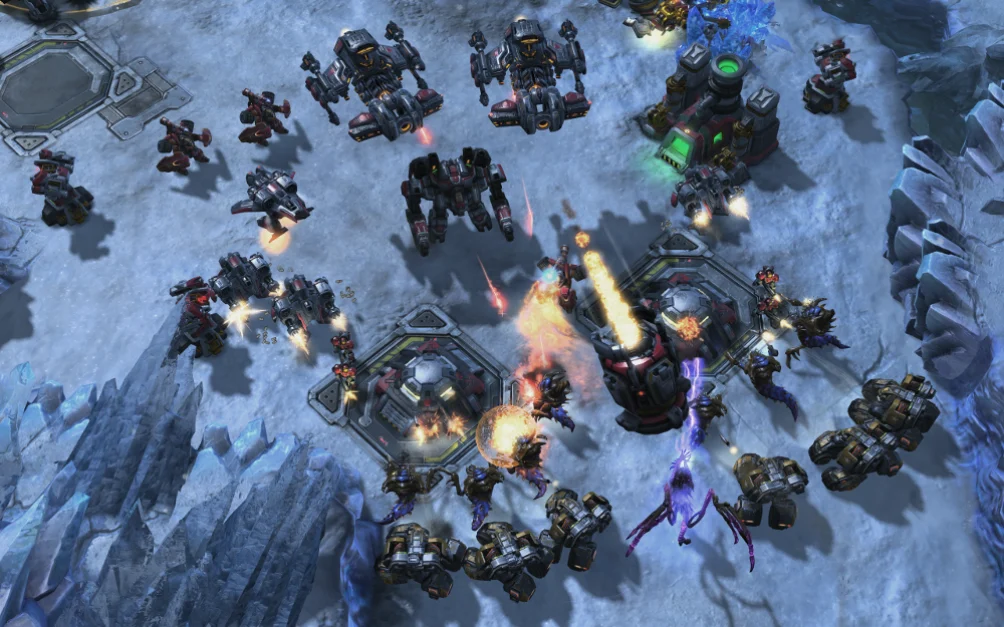
\includegraphics[width=0.8\textwidth]{Cap1/starcraft2.png}
    \caption{A picture of the StarCraft 2 game. Its possible to see a clash between units of Zerg and Terran factions. Credit: Blizzard Entertainment (\url{https://blizzard.com/}).}
    \label{fig:starcraft_2_game}
\end{figure}

What every one of these results leaves untouched, however, is the body.  A
simulated agent issues an action and the action simply happens; a physical one
must produce torques that move mass, manage balance and contact, and recover
when the world reacts in ways no rule foresaw.  This last frontier --- continuous
sensorimotor control on real hardware --- is where progress is now most striking.
Fittingly for a World Cup year, Boston Dynamics has recently demonstrated its
Atlas humanoid performing soccer skills that demand exactly this kind of
dynamic, whole-body coordination on real hardware.

\begin{figure}[h]
    \centering
    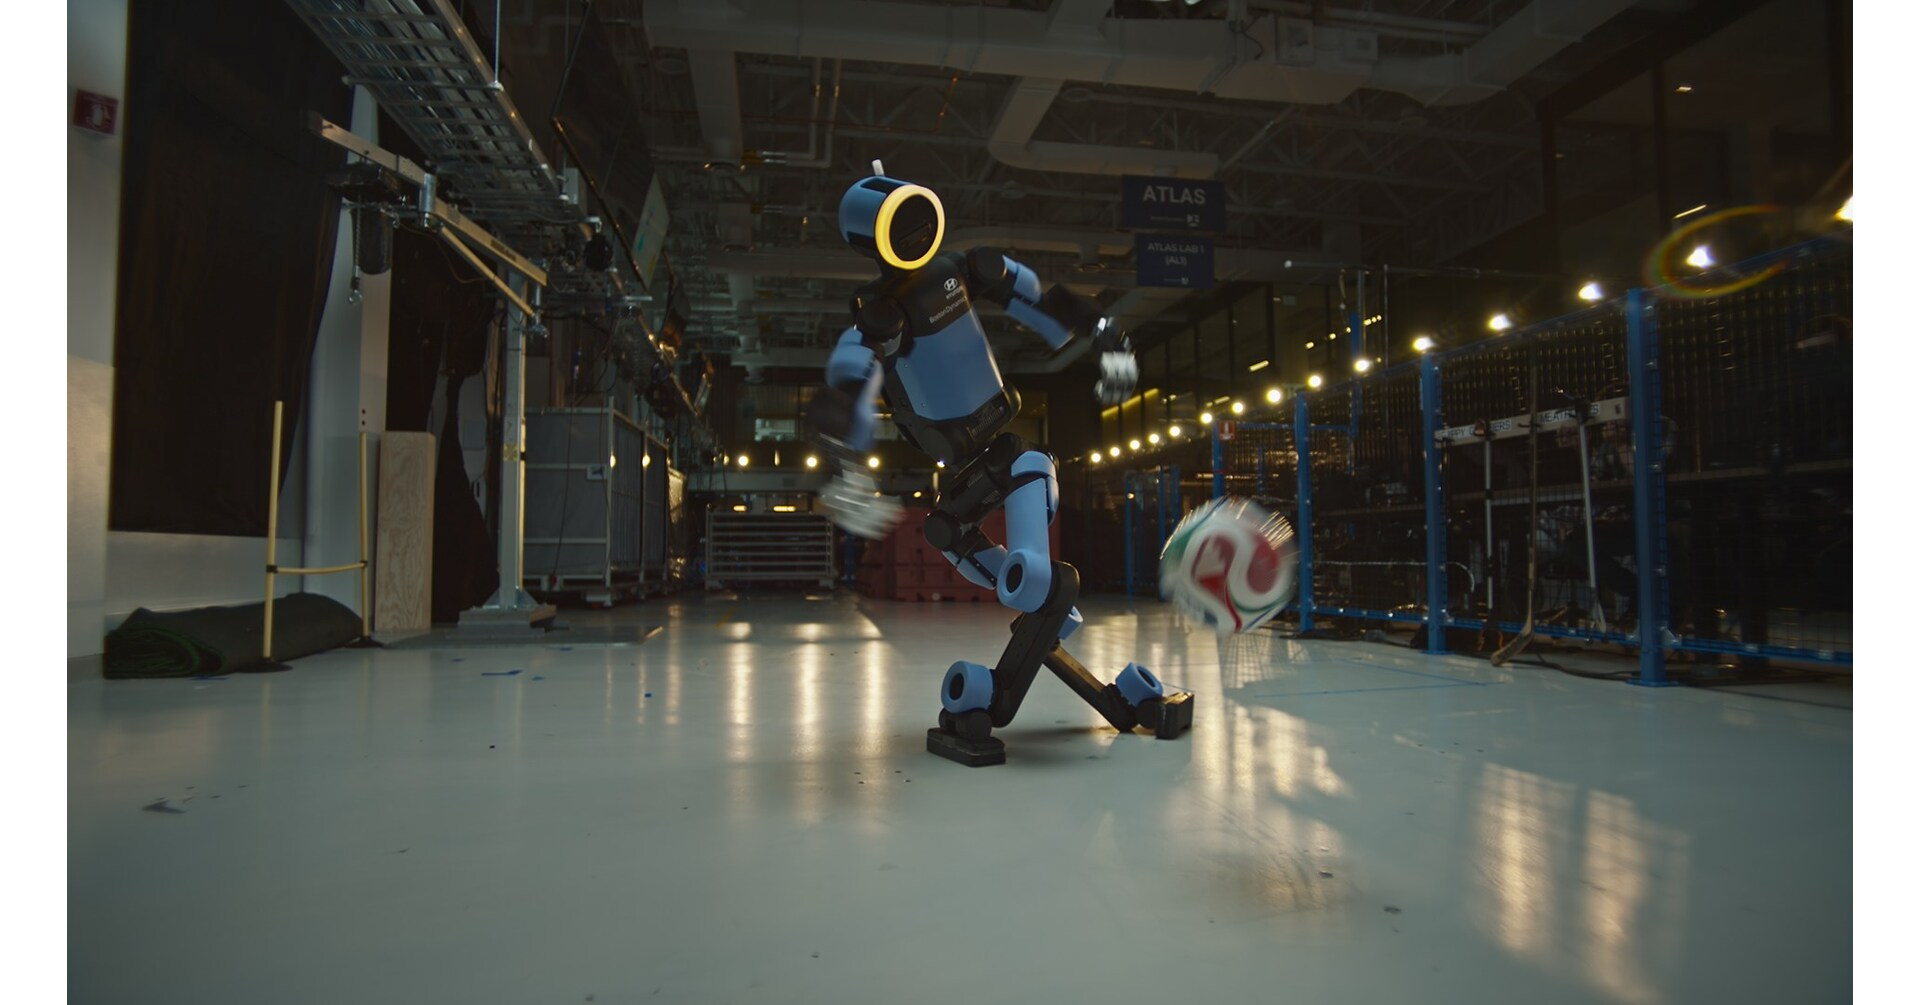
\includegraphics[width=0.8\textwidth]{Cap1/atlas_rabona.png}
    \caption{Picture of a pre-World Cup 2026 marketing stunt for the Boston Dynamics Atlas robot.
    The robot can be seen doing a "Rabona", also known as "chute de letra" in Portuguese.
    Credit: Hyundai and Boston Dynamics (\url{https://bostondynamics.com/atlas}).}
    \label{fig:atlas_rabona}
\end{figure}

Robot soccer occupies a particularly attractive position in this landscape.
It draws together, in one compact and well-defined domain, the threads pulled
apart above: continuous control, real-time decision-making, multi-agent
cooperation, and adversarial competition.  It is cheap enough to simulate at
scale, yet the underlying decision problem remains genuinely hard --- which is
precisely what makes it a demanding benchmark for techniques whose ultimate
target is the physical world.

% ------------------------------------------------------------------
\section{Contextualization}
% ------------------------------------------------------------------

In the context of Robot Soccer, various robotics leagues and competitions have surged in the last decades.
One of the popular leagues in Brazil is the IEEE Very Small Size Soccer (\gls{vsss}),
category in which two teams of
differential-drive robots play on a flat field.  A camera mounted above the
field estimates the positions of all robots and the ball; an off-board computer
processes these estimates and sends wheel-speed commands to each robot via
radio.  In the 3v3 format considered here, each team has three homogeneous
robots and no kicking mechanism, so effective team behavior must arise from
ball conduction, positioning, and coordinated movement.
Figure~\ref{fig:vsss_game_diagram} shows the common IEEE VSSS game setup.

\begin{figure}[ht]
    \centering
    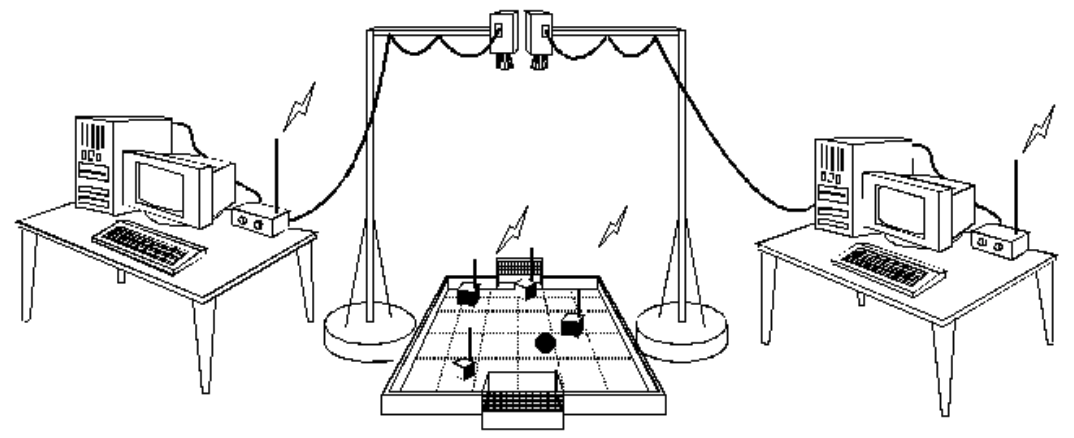
\includegraphics[width=0.82\linewidth]{Cap1/vsss_game.png}
    \caption{IEEE VSSS game set. Credit:~\cite{ieee_vsss_rules}.}
    \label{fig:vsss_game_diagram}
\end{figure}

The ITAndroids \gls{vsss} team currently relies on a classical robotics stack
for strategy, path planning, and low-level control — a hierarchy of carefully
hand-crafted rules and heuristics that govern how each robot navigates the
field and responds to game events. Figure~\ref{fig:vss_robots} shows a picture of the ITAndroids robots and the overhead-vision marker. This stack performs well in practice but
has fundamental limitations.  Rule-based strategies are designed for a finite
set of anticipated situations and do not automatically improve with more
data or competition experience.  Adapting them to a new opponent or a changed
team composition requires manual re-engineering.

\begin{figure}[ht]
    \centering
    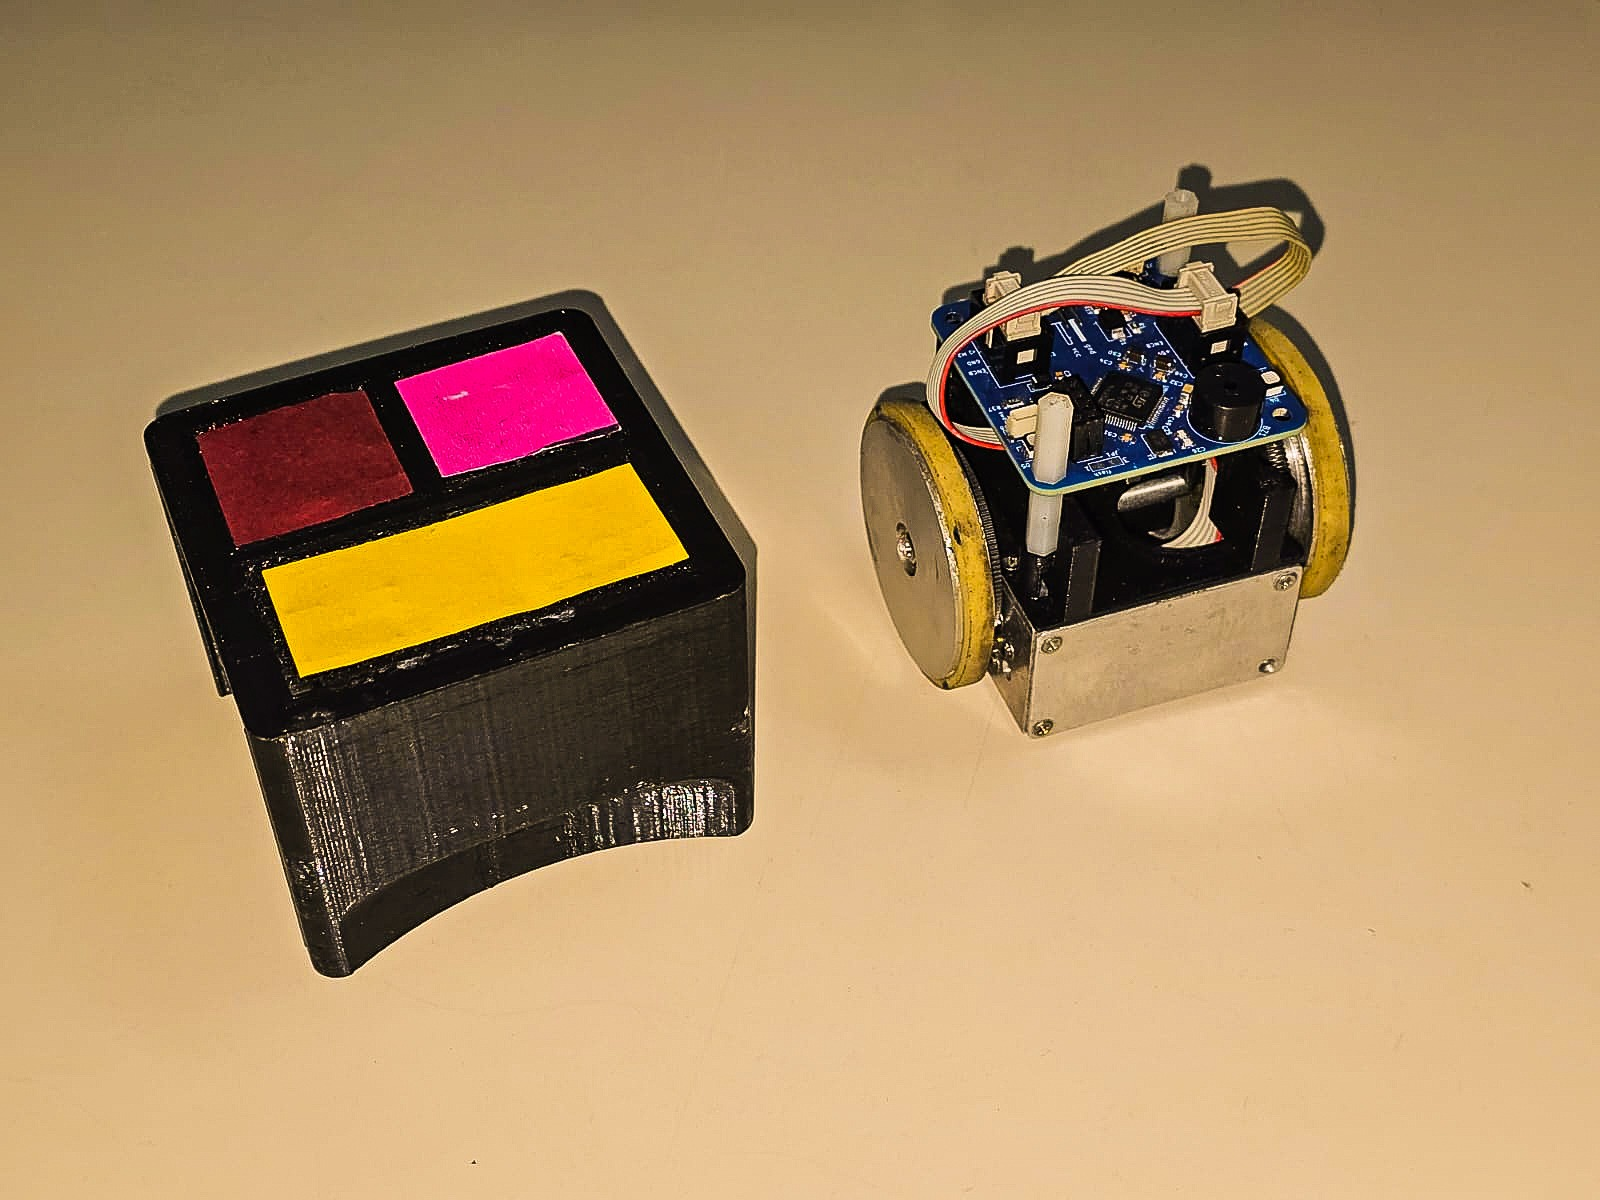
\includegraphics[width=0.75\textwidth]{Cap1/vss.jpeg}
    \caption{ITAndroids \gls{vsss} robots and overhead-vision marker.}
    \label{fig:vss_robots}
\end{figure}

The potential of learned strategies for this domain has been demonstrated by
a series of prior works, each addressing a different scope. \textcite{bassani2020}
developed an open RL framework for \gls{vsss} and showed that
a trained single-agent policy could match the level of human-designed
strategies, reaching fourth place at the 2019 Latin American Robotics
Competition (LARC). \textcite{medeiros2020} applied Proximal Policy Optimization (\gls{ppo})
with curriculum learning to teach a single robot to intercept the ball in the
presence of an opponent, outperforming both handcrafted baselines and agents
trained without the curriculum.  \textcite{tg_thay} extended
this framework to penalty kicks, achieving conversion rates substantially above
the team's existing kicker.  Subsequent work by \textcite{master_thay} moved to an adversarial multi-agent setting, studying how
different opponent-sampling strategies affect the quality of the learned policy
in penalty-kick scenarios.  \textcite{brandao2022} went
further, applying \gls{ppo} with self-play to a full 3v3 team, simultaneously
learning control and strategy, and demonstrating that the resulting policy
could defeat the best available heuristic opponent with an 84\% win
rate.

This thesis is the natural next step in that line of work.  Where \textcite{brandao2022}
showed that 3v3 multi-agent learning is feasible, the
experiments there were constrained by the cost of collecting enough useful
experience.  The central question this work addresses is what becomes possible
when training can both generate more transitions per wall-clock second and make
better use of the situations it samples.

% ------------------------------------------------------------------
\section{Objective}
% ------------------------------------------------------------------

The objective of this work is to reduce one of the main practical barriers that
still separates reinforcement-learning research in \gls{vsss} from routine use
inside the ITAndroids development cycle.  The team already has a sequence of
works showing that learned policies can perform meaningful soccer behaviors,
from isolated skills to complete 3v3 control.  However, training and evaluating
these policies remains expensive: each experiment requires a large number of
simulated interactions, and the existing simulator architecture limits how
quickly those interactions can be produced.

This work therefore concentrates on the infrastructure needed to make such a
strategy learnable.  An accelerated \gls{vsss} simulator is developed and
integrated into an end-to-end \gls{ppo} training loop for a centralized joint
team policy.  The resulting baseline allows the simulator to be measured in a
real learning setting and establishes the foundations for the sample-selection
and multi-agent extensions that follow in TG-2.

% ------------------------------------------------------------------
\section{Literature Review}
% ------------------------------------------------------------------

This section reviews the work most relevant to a learning-based approach to
3v3 \gls{vsss}.  It proceeds from the broad milestones that established deep
reinforcement learning as a viable tool for strategic control, through the
specific body of \gls{vsss} research developed within the ITAndroids team, to
accelerated simulation and sample efficiency improvements.

\subsection{Deep Reinforcement Learning in Games and Robotics}

The modern interest in deep reinforcement learning for sequential
decision-making was catalyzed by a sequence of results in games of increasing
complexity.  AlphaGo defeated a professional Go player by combining
deep neural networks with Monte Carlo tree search~\cite{silver2016mastering},
and its successor AlphaGo Zero reached superhuman play through self-play
alone, learning without any human game data~\cite{silver2017mastering}.  These
results established two ideas central to this work: that a single learned
function can encode sophisticated strategy, and that self-play can generate the
training signal needed to reach it.

Subsequent work scaled these ideas to real-time, multi-agent, partially
observable settings.  OpenAI Five coordinated a team of five agents to defeat
human champions at the video game Dota~2~\cite{berner2019dota}, and AlphaStar
reached Grandmaster level in StarCraft~II by training a league of continually
adapting agents, each representing a distinct strategy, to prevent the policy
from overfitting to a single style of play~\cite{starcraft_marl}.  The
league-training idea — that competitive robustness requires facing a diverse
population of opponents rather than only the latest policy — directly informs
the self-play design considered in this work.

\subsection{Reinforcement Learning in IEEE VSSS}

Within the \gls{vsss} category specifically, a focused body of work — much of it
produced within the ITAndroids team — has progressively expanded the role of
reinforcement learning from isolated skills toward full-team play.

\textcite{medeiros2020} introduced reinforcement learning to \gls{vsss} strategy
by training a single robot, with \gls{ppo}, to intercept and control the ball in
the presence of an opponent.  Two design choices from that
work recur throughout the subsequent literature and in this thesis.  First, the
action space was taken as the robot's wheel speeds rather than a target position
handed to an external controller, which forces the policy to solve the planning
and control problems jointly.  Second, because goal events are too sparse to
drive early learning, the reward was shaped with intermediate terms and training
was organized as a curriculum, with the agent and ball beginning close together
and gradually separating and the opponent initially stationary and later set in
motion.  Agents trained with this curriculum matched or outperformed both agents
trained without it and the team's classical heuristics, establishing \gls{ppo}
with curriculum learning as a strong baseline for the domain.

\textcite{master_thiago} later extended this framework, broadening
from a single defensive skill to four scenarios — intercepting the ball on the
player's side and recovering it to the opponent's side, each with and without an
opponent — and introducing cooperative self-play, in which each agent carries a
copy of the same network and learns to coordinate with itself rather than treat
its copy purely as an adversary. This is, to the author's
knowledge, the first work to combine self-play with \gls{ppo} in \gls{vsss}, and
its scenario-based curriculum and shared-network design are direct antecedents
of the two-stage, symmetry-aware approach taken here.

\textcite{tg_Yamane} addressed a different role and a different challenge: a learned
goalkeeper policy and, crucially, its transfer to physical
hardware.  Where the earlier works evaluated policies only in
simulation, this thesis confronts the reality gap between the simulator and the
real robot, treating line-following control and decision-making under real
sensing and actuation noise.  Its treatment of sim-to-real transfer frames the
domain-randomization and noise-injection considerations that the present work
defers to its own future-work agenda.

\textcite{master_thay} moved the framework into an explicitly adversarial,
multi-agent regime, studying penalty-kick scenarios in which an attacker and a
goalkeeper are trained against each other.  The central
question of that work is how to choose the opponent during self-play.  It
formalizes a family of opponent-sampling strategies that differ in how much of
the training history they draw from — for instance, sampling uniformly from all
past versions of the opponent, from only the most recent half, or from a fixed
recent window — and analyzes how this choice affects the robustness and quality
of the learned policy.  This is precisely the design space that the second
curriculum stage of the present work must navigate, and Baldão's analysis is the
most directly applicable guidance available for it.

Beyond the ITAndroids line, \textcite{bassani2020} developed an open
reinforcement-learning framework for \gls{vsss} and demonstrated sim-to-real
transfer of trained policies, with a resulting team placing competitively at the
2019 Latin American Robotics Competition.  Closest in spirit
to this thesis, \textcite{brandao2022} trained a full 3v3 team with multi-agent
\gls{ppo} and self-play, using a shared policy across the three homogeneous
robots and a centralized data-collection scheme, and reported a policy capable
of defeating the strongest available heuristic opponent.
That work establishes that full-team 3v3 learning is feasible; the present
work takes that feasibility as its starting point and asks what becomes possible
once the simulation-throughput and sample-efficiency constraints under which it
operated are relaxed.

\subsection{Accelerated Simulation for Reinforcement Learning}

On-policy algorithms such as \gls{ppo} consume a large volume of fresh
environment transitions, which makes simulation throughput a primary determinant
of training cost.  The \gls{vsss} works above run physics on the \gls{cpu} and
communicate with the learner across a process boundary, an architecture whose
throughput scales poorly with the number of parallel environments.

A recent direction addresses this by relocating the environment onto the
hardware accelerator.  Frameworks such as Brax express rigid-body physics as
differentiable, batched array operations that execute on \gls{gpu}, allowing
thousands of environments to be stepped simultaneously and bringing the
simulator and the learner onto the same device~\cite{brax2021}.  In the robot
soccer context specifically, \textcite{scaling_marl_2d} built a custom 2D environment
whose physics is expressed as simple vectorizable operations and reported
throughput one to two orders of magnitude higher than a wrapped general-purpose
simulator for the same task, demonstrating that a purpose-built
batched environment can dramatically reduce training time precisely because it
avoids the overhead of a general engine.  The simulator developed in this work
follows this paradigm, applying it to the \gls{vsss} domain.

\subsection{Prioritized Experience and Scenario Selection}

A complementary way to reduce training cost is to improve the value of each
transition rather than the rate at which transitions are produced.  Prioritized
Experience Replay~\cite{schaul2016per} established that, in off-policy learning,
replaying transitions in proportion to their temporal-difference error learns
faster than uniform replay.  Prioritized Level Replay (\gls{plr}) extends this
intuition to the selection of \emph{which situations to play} rather than which
past transitions to revisit: it scores environment configurations by an estimate
of their future learning potential and biases the agent's experience toward the
configurations expected to be most informative, inducing an implicit curriculum
without any predefined ordering of difficulty~\cite{prioritized_level_replay}.  The sampler
proposed in this work adapts this principle to \gls{vsss}, treating each
initialized game situation as a level whose priority is derived from the
policy's recent value-prediction error.

The same selection problem also appears in multi-agent self-play.  AlphaStar's
league training, for example, did not train only against the latest policy; it
maintained a population of agents so that the learner faced varied opponents and
did not overfit to a single strategy~\cite{starcraft_marl}.  In this work,
\gls{plr} addresses the analogous question on the environment side: which game
situations should the current policy experience next?

% ------------------------------------------------------------------
\section{Contributions}
\label{sec:contributions}
% ------------------------------------------------------------------

This work is organized around two costs that limit large-scale reinforcement
learning in \gls{vsss}: throughput, or how many fresh transitions can be
produced per second, and sample efficiency, or how informative those transitions
are for the current policy.  The first cost is addressed directly by moving the
simulator onto the accelerator.  The second is addressed in TG-1 by establishing
the training baseline and initialization interface on which the
prioritized-level-replay sampler will operate in TG-2.

The two main TG-1 contributions are therefore:

\begin{itemize}
    \item A JAX-based, GPU-parallel simulator for 3v3 \gls{vsss}, built
    around batched physics and accelerator-friendly rollout loops.  The
    simulator is designed to step thousands of independent game instances
    simultaneously on a single device, eliminating the inter-process
    communication overhead present in all existing \gls{vsss} training
    pipelines.

    \item A policy-training baseline for sample-efficient extensions: a
    centralized joint policy
    trained from scratch to control a 3v3 \gls{vsss} team using the new
    simulator, with learning curves showing that the infrastructure supports
    reliable policy improvement and characterizing the role of initialization
    strategy in the learning process.  These results motivate the
    \gls{plr} sampler and provide the comparison point for its TG-2 evaluation.
\end{itemize}

The TG-1 policy is deliberately centralized: a single network observes the
global game state and commands all three allied robots simultaneously.  This
controlled baseline isolates the throughput and sample-selection contributions
from the additional complexity of per-robot decentralization, full self-play,
and symmetry-aware data augmentation.

This work also contributes to the relatively limited literature on applying
deep \gls{rl} to full-team decision-making and control in the IEEE \gls{vsss}
league, and aligns with the ITAndroids team's mission of advancing and
disseminating knowledge in robotics and artificial intelligence.

% ------------------------------------------------------------------
\section{Outline of this Work}
% ------------------------------------------------------------------

The remainder of this work is organized as follows:
\begin{itemize}
  \item \textbf{Chapter~2} describes the IEEE \gls{vsss} domain, the differential-drive robot model, and the existing simulators used in the community and their limitations for large-scale \gls{rl} training.
  \item \textbf{Chapter~3} covers the machine-learning background: reinforcement learning fundamentals, \gls{ppo}, curriculum learning, prioritized level replay, multi-agent self-play, symmetry exploitation, and GPU-accelerated simulation.
  \item \textbf{Chapter~4} defines the proposed methodology, including the multi-agent \gls{mdp} formulation, policy architecture, and simulator design.
  \item \textbf{Chapter~5} reports preliminary TG-1 results, focusing on measured simulator throughput, interface validation and two simple example policy training experiments, as well as some of the discussion regarding the role of planned improvements in TG-2.
  \item \textbf{Chapter~6} summarizes TG-1 and defines the roadmap toward TG-2.
\end{itemize}

\chapter{IEEE Very Small Size Soccer}
% ============================================================
%  THEORETICAL BACKGROUND — IEEE VSSS DOMAIN
%  Complete text for the three sections.
%  (The first two sections are lightly revised from your draft;
%   the third is written from scratch.)
% ============================================================

This chapter covers the IEEE VSSS domain, the differential-drive robot model, and the existing simulators used in the community, identifying the architectural constraints that motivate the GPU-accelerated approach taken in this work.

% ------------------------------------------------------------------
\section{The IEEE VSSS Domain}
% ------------------------------------------------------------------

IEEE Very Small Size Soccer (\gls{vsss}) is a Robot Soccer category in which two teams
of small differential-drive robots compete on a flat field.  The robots are
remotely controlled by a computer set by each team that receives the state of the
game from a camera set over the field and sends wheel-speed commands by radio~\parencite{robocore_vsss_rules}.  Human
intervention is not allowed during regular play, so the control system must
close the loop from perception to decision-making and actuation.

Compared with larger Robot Soccer leagues, \gls{vsss} has relatively simpler
physics: rigid (no geometry-altering controllable joints) robots, a ball, wall collisions, friction, and no kicking
mechanism.  This simplicity makes the domain specially attractive for reinforcement
learning because it can be simulated at high computational efficiency.
At the same time, the task is not trivial: a team must conduct the ball by contact, coordinate the motion of multiple robots, avoid blocking itself, defend its goal, and exploit opportunities created by the opponent.

The match for a 3v3 category variant takes place on a rectangular field of dimensions
$1.50\,\text{m} \times 1.30\,\text{m}$ (excluding the goal areas), with one
goal centered on each of the shorter sides.  Figure~\ref{fig:field} shows the
regulation layout for the 3v3 field in centimetres (goals, penalty areas, centre circle, and chamfered corners).  An overhead camera feeds a vision system that estimates the position of the ball and the pose (position and orientation) of every robot; those estimates are then consumed by the decision-making stack (strategy, path planning, and low-level control).
In real hardware, the whole pipeline (vision and decision-making) runs inside a computer set by each team that
issues wheel-speed commands over radio, so all computation is centralized.

\begin{figure}[ht]
    \centering
    \resizebox{0.88\linewidth}{!}{%
        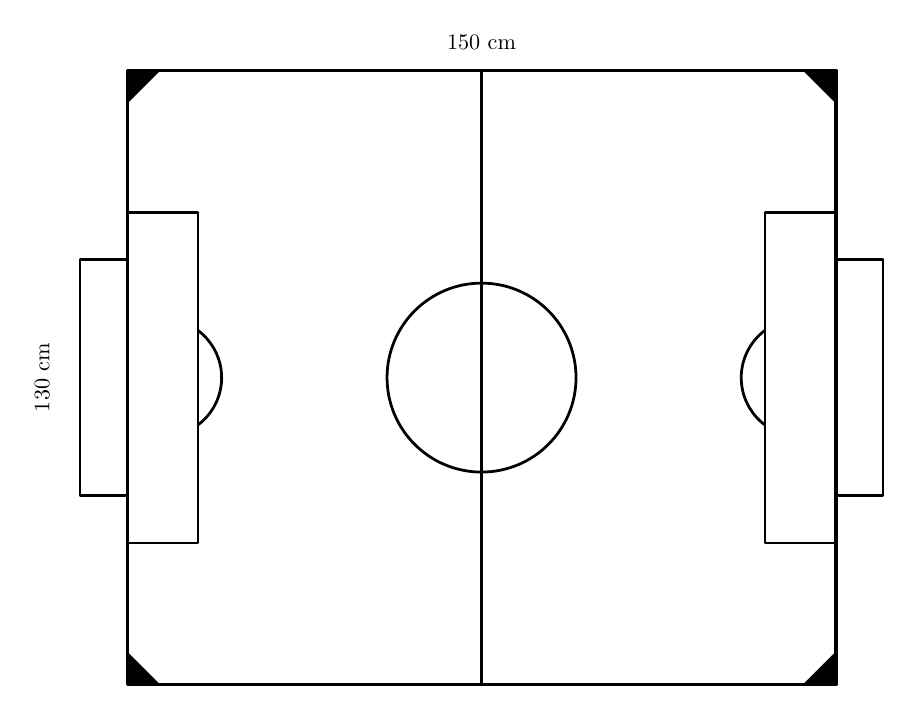
\begin{tikzpicture}[scale=0.06, line cap=round, line join=round]

  % Dimensions: field 150cm x 130cm
  \def\W{150}
  \def\H{130}
  
  % Outer field
  \draw[line width=1.2pt] (0,0) rectangle (\W,\H);
  
  % Chamfered black corners, 7cm
  \foreach \x/\y/\xa/\ya/\xb/\yb in {
  0/0/7/0/0/7,
  150/0/143/0/150/7,
  0/130/7/130/0/123,
  150/130/143/130/150/123}
  {
    \fill (\x,\y) -- (\xa,\ya) -- (\xb,\yb) -- cycle;
  }
  
  % Center line
  \draw[line width=1pt] (75,0) -- (75,\H);
  
  % Center circle, diameter 40cm
  \draw[line width=1pt] (75,65) circle (20);
  
  % Goals
  \draw[line width=1pt] (-10,40) rectangle (0,90);
  \draw[line width=1pt] (\W,40) rectangle (\W+10,90);
  
  % Goal areas / boxes
  \draw[line width=1pt] (0,30) rectangle (15,100);
  \draw[line width=1pt] (\W-15,30) rectangle (\W,100);
  
% --- Penalty arcs via circumcenter / 3 points ---

% Left arc: start (20,55), through (15,65), end (20,75)
\tkzDefPoint(15,55){LA}
\tkzDefPoint(20,65){LB}
\tkzDefPoint(15,75){LC}
\tkzCircumCenter(LA,LB,LC)\tkzGetPoint{LO}
\tkzDrawArc[line width=1pt](LO,LA)(LC)

% Right arc: start (130,75), through (135,65), end (130,55)
\tkzDefPoint(135,75){RA}
\tkzDefPoint(130,65){RB}
\tkzDefPoint(135,55){RC}
\tkzCircumCenter(RA,RB,RC)\tkzGetPoint{RO}
\tkzDrawArc[line width=1pt](RO,RA)(RC)
  
  % Small marks / dots
  % \foreach \x/\y in {
  % 17.5/25, 57.5/25,
  % 17.5/105, 57.5/105,
  % 92.5/25, 132.5/25,
  % 92.5/105, 132.5/105}
  % {
  %   \draw[line width=0.8pt] (\x,\y) circle (1.2);
  % }
  
  % Cross markers
  % \foreach \x/\y/\txt in {
  % 37.5/25/{\textbf{\color{red}(FB)}},
  % 37.5/65/{\textbf{\color{red}(PK, FK)}},
  % 37.5/105/{\textbf{\color{red}(FB)}},
  % 112.5/25/{\textbf{\color{red}(FB)}},
  % 112.5/65/{\textbf{\color{red}(PK, FK)}},
  % 112.5/105/{\textbf{\color{red}(FB)}}}
  % {
  %   \draw[line width=1pt] (\x-2,\y) -- (\x+2,\y);
  %   \draw[line width=1pt] (\x,\y-2) -- (\x,\y+2);
  %   \node[scale=0.75] at (\x,\y+7) {\txt};
  % }
  
  % Optional coordinate labels
  \node[scale=0.8] at (75,136) {150 cm};
  \node[scale=0.8, rotate=90] at (-18,65) {130 cm};
  
  \end{tikzpicture}
%
    }
    \caption{IEEE VSSS field (top view, dimensions in cm).  Goals are
    $40$\,cm wide; penalty areas and centre markings follow the competition
    ruleset.}
    \label{fig:field}
\end{figure}

The 3v3 setting considered in this thesis increases the multi-agent nature
of the problem.  A single policy action can be evaluated only in the context
of the other allied robots and the opponent team.  This creates both
cooperative credit-assignment challenges and adversarial non-stationarity,
which the training methodology must address.

% ------------------------------------------------------------------
\section{Differential-Drive Robot Model}
% ------------------------------------------------------------------

Each \gls{vsss} robot can be modeled as a differential-drive body with two
independently actuated wheels.  A common kinematic mapping from body velocity
to wheel angular velocities~\cite{franzoni2017} is:

\begin{equation}
    \gls{wheel_speed_left} = \frac{2\gls{linear_velocity} - \gls{wheel_base}\,\gls{angular_velocity}}{\gls{wheel_diameter}},
    \qquad
    \gls{wheel_speed_right} = \frac{2\gls{linear_velocity} + \gls{wheel_base}\,\gls{angular_velocity}}{\gls{wheel_diameter}},
    \label{eq:diff_drive}
\end{equation}

where \gls{linear_velocity} is the desired linear velocity of the robot
center, \gls{angular_velocity} the desired angular velocity,
\gls{wheel_base} the distance between the wheel contact points,
\gls{wheel_diameter} the wheel diameter, and \gls{wheel_speed_left},
\gls{wheel_speed_right} the resulting left and right wheel angular
velocities.
This mapping is important because it defines the interface between the policy
and the simulator.  The policy may output wheel speeds directly, or it may
output higher-level $(v,\omega)$ commands that are converted into wheel
speeds before stepping the physics.  Direct wheel-speed actions are closer
to the hardware interface, while body-velocity actions can simplify learning
by exposing a more structured control space.

In the VSSS literature, both conventions have been used.
\cite{tg_thiago} and subsequent ITAndroids works adopt body
velocities as the policy output, converting them to wheel commands via
Equation~\eqref{eq:diff_drive} before dispatching to the simulator.
\cite{tg_thay} instead parameterize actions directly as a tuple of
left and right wheel speeds, arguing that the end-to-end formulation reduces
the gap between simulated commands and actual hardware actuation.  In either
case the robot is treated as a rigid cube that moves according to
Equation~\eqref{eq:diff_drive}, with friction and wall collisions handled by
the physics engine.

% ------------------------------------------------------------------
\section{Existing Simulators and Their Limitations for RL}
% ------------------------------------------------------------------

Because reinforcement learning algorithms require orders of magnitude more
interaction steps than classical approaches to converge, it is not practical
to train directly on physical hardware — doing so would quickly degrade the
robots' mechanical components and impose severe time constraints on
experimentation.  Simulation is therefore a necessary prerequisite, and the
choice of simulator has a direct bearing on how ambitious the training
methodology can be.

\subsection{The Conventional Architecture: ODE-Based Simulators}

The most established simulators in the VSSS community share a common
architectural pattern: a physics engine based on the \emph{Open Dynamics
Engine} (\gls{ode}). Written in C++, that runs as a standalone process and exposes
its state to external agents through socket messages.  ODE is an open-source
library for simulating rigid-body dynamics that requires only the geometry and
inertial parameters of each body as input, rather than manually derived
equations of motion \cite{smith2001}.  This makes it relatively
straightforward to replicate the VSSS scenario — a handful of cubic robots, a
spherical ball, and a bounded rectangular field.

Two simulators of this kind were mainly used in the VSSS analyzed works: the first,
developed by ITAndroids and used in prior works from the
group~\parencite{tg_thiago,tg_thay,master_thay}, combines ODE for physics
with the Object-Oriented Graphics Rendering Engine (OGRE) for visualization.
It operates at a fixed iteration rate of 60\,Hz and communicates with the
agent binaries through synchronous TCP socket packages built on the ZeroMQ
library.  To mimic real-world conditions, the simulator can inject additive
Gaussian noise into the position and orientation estimates it reports, and
can simulate communication delay by queuing observation packets and releasing
them with a configurable lag.  Figure~\ref{fig:itandroids_simulator} shows the
simulator rendering a penalty situation.

\begin{figure}[ht]
    \centering
    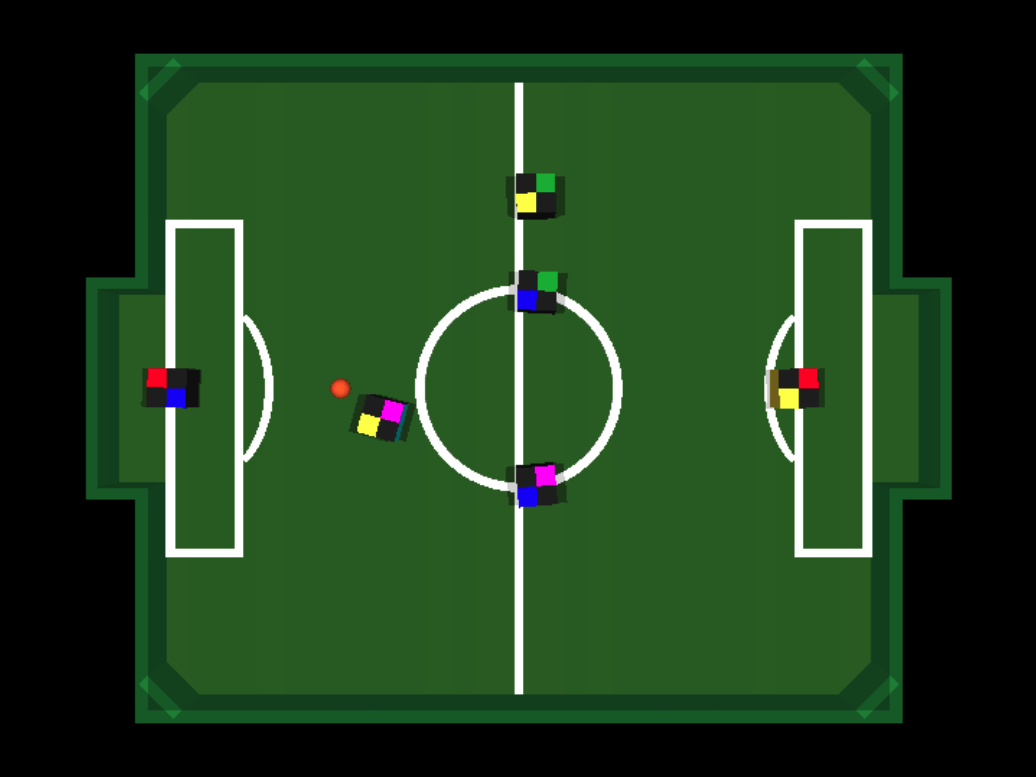
\includegraphics[width=0.82\linewidth]{Cap2/server.png}
    \caption{Screenshot of the ITAndroids ODE-based simulator in a penalty
    situation, with attacking and defending robots positioned around the ball.
    Image credit:~\parencite{master_thay}.}
    \label{fig:itandroids_simulator}
\end{figure}

The second, FIRASim~\cite{firasim2019}, was adapted from the RoboCup Small
Size League simulator grSim and is the reference environment used by many of the Brazilian VSSS simulated competitions.  It also uses ODE for
physics but is a different implementation, with known behavioral differences:
it does not enforce velocity limits on robots and omits friction in certain
contact configurations.  FIRASim uses asynchronous
UDP communication rather than TCP, and does not include built-in noise or delay injection.  Figure~\ref{fig:firasim} shows a FIRASim match state.

\begin{figure}[ht]
    \centering
    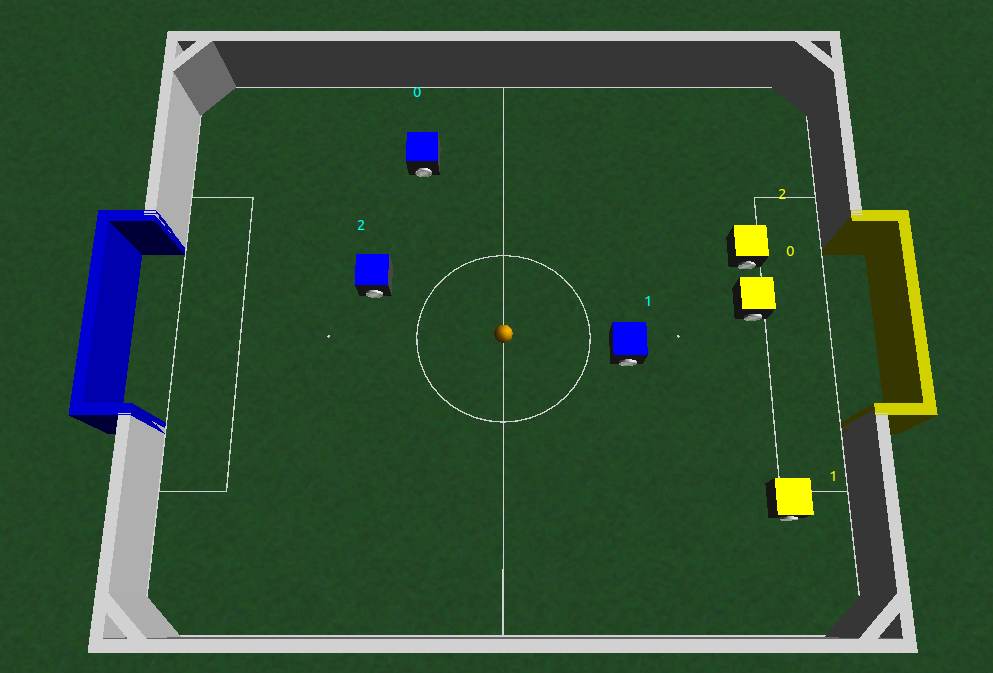
\includegraphics[width=0.82\linewidth]{Cap2/firasim.png}
    \caption{Screenshot of the FIRASim simulator, the ODE-based environment commonly used in Brazilian VSSS simulated competitions. Credit:~\parencite{firasim2019}.}
    \label{fig:firasim}
\end{figure}

Both simulators expose an interface in which the agent processes are entirely
separate from the physics process.  At each timestep, the simulator broadcasts
the current game state (robot poses, velocities, and ball state) to both teams,
waits for them to respond with desired wheel speeds, updates the physics, and
then repeats.  This synchronous, round-trip structure means that the simulator and the agent
processes are tightly coupled in time even though they run independently.
Gym-compatible wrappers have been built on
top of both engines to standardize the observation and action spaces and to
allow interchangeable use with general RL toolkits, following \parencite{bassani2020}.

\subsection{The Throughput Bottleneck}

The multi-process, socket-based architecture described above introduces a
fundamental throughput bottleneck that becomes critical when scaling RL
training.  Every environment step involves serializing the game state into a
network packet, crossing an inter-process communication boundary, waiting for
the agent process to deserialize, compute, and serialize its reply, and then
crossing the boundary again.  Even on a single machine, this round-trip imposes
a non-negligible per-step latency that caps the number of environment steps per
second, regardless of how fast the underlying physics computation is.

\textcite{medeiros2020} addressed this partially by merging the simulator and
the agent processes into a single executable, eliminating the socket round
trip.  \textcite{master_thay} subsequently reused this adaptation, further
bridging the C++ simulator with a Python RL stack via gRPC.  While these
modifications reduced coordination overhead, the underlying single-threaded
simulation remained inherently sequential: one environment steps at a time,
on CPU.

Table~\ref{tab:legacy_throughput} summarises simulation throughput for two
representative ITAndroids RL works that trained on the ODE-based engine
described above.  No prior VSSS work measures simulator throughput directly;
the values are derived from wall-clock training durations reported in the
original monographs.

\begin{table}[ht]
    \centering
    \caption{Simulation throughput in prior ITAndroids RL works on the
    ODE-based engine, derived from reported wall-clock training durations.
    All figures represent RL control steps per second per simulator instance
    (15\,Hz control rate, 4-frame action repeat over 60\,Hz physics).}
    \label{tab:legacy_throughput}
    \begin{tabular}{lrr}
        \toprule
        \textbf{Work} & \textbf{Environments} &
        \textbf{Steps/s} \\
        \midrule
        \cite{tg_thay} &
            1 & $63$\tnote{a} \\
        \cite{master_thiago} &
            4 & $378$\tnote{b} \\
        \bottomrule
    \end{tabular}

    \medskip
    \begin{minipage}{\linewidth}\small
        \textsuperscript{a}~Derived from Table~6.1 of~\cite{tg_thay}:
        subtask \textit{LFG-SG} trained for $5\times10^{6}$ steps in an
        average wall-clock time of 21\,h\,28\,min per agent across 64
        independent runs (one simulator instance per agent).
        $5{\times}10^{6}\,/\,(21.47\times3600)\approx64.7$\,steps/s; the
        three LFG subtasks yield consistent estimates of $62$--$65$\,steps/s,
        rounded here to approximately $63$\,steps/s.

        \medskip
        \textsuperscript{b}~Derived from Section~6 of~\cite{master_thiago}:
        $34\times10^{6}$ timesteps completed in 25\,h of wall-clock time
        (fragmented-CL condition), with 16 agents each driving 4 simulator
        processes in parallel.  Interpreting the 34\,M budget as per-agent
        gives $34{\times}10^{6}\,/\,(25\times3600)\approx378$\,steps/s per
        agent; dividing by the 4 parallel simulator instances per agent
        yields approximately $94$\,steps/s per instance.
    \end{minipage}
\end{table}

The consequences become apparent at scale.  \textcite{brandao2022} managed
to run 200 parallel instances of a MuJoCo-based VSSS simulation for their
multi-agent PPO training, a significant improvement, but even so, the
simulation ran on CPU, with the physics engine unable to exploit the
parallelism available on modern hardware accelerators.  In the broader robot
soccer literature, \textcite{scaling_marl_2d} demonstrated that a purpose-built
2D environment whose physics is expressed as simple, vectorizable operations
could achieve throughput one to two orders of magnitude higher than
MuJoCo-backed alternatives for the same number of players, precisely because
it allowed the simulation loop to bypass the CPU bottleneck.

\subsection{Implications for This Work}

The gap between what existing VSSS simulators can provide and what an
ambitious multi-agent training regime requires is the central motivation for
the simulator developed in this thesis.  Training a 3v3 cooperative policy
from scratch with PPO, a two-stage curriculum, and self-play requires tens or
hundreds of millions of environment steps to converge; the ITAndroids prior
works were constrained to much smaller timestep budgets partly because of this
constraint.

The simulator proposed here takes a different approach.  Rather than wrapping
a C++ physics engine and mediating access through sockets, it expresses the
entire VSSS physics (rigid-body kinematics, collision detection, and ball
dynamics) as batched array operations that can be compiled and executed
on a \gls{gpu}.  This design makes it possible to step thousands of
independent game instances simultaneously within a single device call,
eliminating inter-process communication and CPU-GPU data transfers from the
critical path.  The physics model is deliberately simpler than a full \gls{ode}
simulation: it captures the aspects of the game that matter most for learning
(differential-drive kinematics, ball-robot contact, wall collisions, and
friction) while sacrificing details that would prevent vectorization or require
variable-time-step integration.  A \emph{faithful-enough} simulation that
supports policy transfer to real hardware is the goal; domain randomization
and noise injection address the remaining sim-to-real gap separately.

\chapter{Machine Learning}
% ============================================================
%  THEORETICAL BACKGROUND — MACHINE LEARNING / RL CHAPTER
%  Drop-in replacement for the seven-section outline.
% ============================================================

\section{Neural Networks}

An artificial neural network is a parametric function approximator built from
layers of interconnected units.  Neural networks are central to this work
because the policy $\pi_\theta$ and the value function $V_w$ are both
represented as neural networks whose parameters are updated by the learning
algorithm.

\subsection{Fundamentals}

The basic building block of a neural network is an artificial neuron, which
computes a scalar output from a vector input $\mathbf{x} \in \mathbb{R}^n$:
%
\begin{equation}
    z = \sigma\!\left(\mathbf{w}^\top \mathbf{x} + b\right),
\end{equation}
%
where $\mathbf{w} \in \mathbb{R}^n$ is a weight vector, $b \in \mathbb{R}$ is
a bias term, and $\sigma : \mathbb{R} \to \mathbb{R}$ is a nonlinear
\emph{activation function}.  Without $\sigma$ the neuron would be a simple
affine transformation; the activation function introduces the nonlinearity
required to represent functions beyond the linear family.  Common choices
include the rectified linear unit $\text{ReLU}(z) = \max(0, z)$, the
hyperbolic tangent $\tanh$, and the logistic sigmoid, each with different
saturation and gradient properties.
Figure~\ref{fig:perceptron} summarizes the data flow for one such unit.

\begin{figure}[ht]
    \centering
    \resizebox{0.75\linewidth}{!}{%
        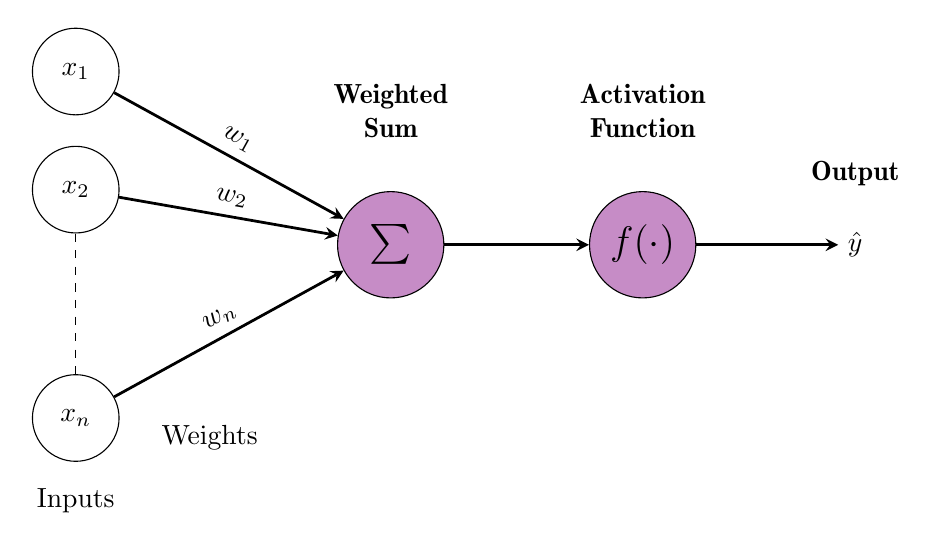
\begin{tikzpicture}[
    node distance=1.8cm,
    neuron/.style={circle, draw, minimum size=1.1cm, font=\bfseries},
    block/.style={circle, draw, fill=violet!45, minimum size=1.35cm},
    arrow/.style={->, >=stealth, line width=1pt},
    label/.style={font=\bfseries}
]

% Inputs
\node[neuron] (x1) at (0,2.2) {$x_1$};
\node[neuron] (x2) at (0,0.7) {$x_2$};
\node[neuron] (xn) at (0,-2.2) {$x_n$};

\draw[dashed] (x2) -- (xn);

\node at (0,-3.25) {Inputs};

% Weighted sum
\node[block] (sum) at (4,0) {\Large $\sum$};
\node[label, align=center] at (4,1.7) {Weighted\\Sum};

% Activation function
\node[block] (act) at (7.2,0) {\Large $f(\cdot)$};
\node[label, align=center] at (7.2,1.7) {Activation\\Function};

% Output
\node[label] (outlabel) at (9.9,0.9) {Output};
\node (out) at (9.9,0) {$\hat{y}$};

% Arrows from inputs
\draw[arrow] (x1) -- node[above, sloped] {$w_1$} (sum);
\draw[arrow] (x2) -- node[above, sloped] {$w_2$} (sum);
\draw[arrow] (xn) -- node[above, sloped] {$w_n$} (sum);

% Arrows between processing nodes
\draw[arrow] (sum) -- (act);
\draw[arrow] (act) -- (out);

% Weights label
\node at (1.7,-2.45) {Weights};

\end{tikzpicture}%
    }
    \caption{Single artificial neuron: weighted sum of inputs $x_i$, bias absorbed
    into weights if a constant input is used, nonlinear activation $\sigma$,
    and scalar output $\hat{y}$ (cf.\ Equation above with $\sigma = f$).}
    \label{fig:perceptron}
\end{figure}

A \emph{multilayer perceptron} (MLP) stacks $L$ layers of neurons.  Writing
$\mathbf{h}^{(0)} = \mathbf{x}$ for the input, each hidden layer computes
%
\begin{equation}
    \mathbf{h}^{(l)} = \sigma\!\left(W^{(l)}\mathbf{h}^{(l-1)} + \mathbf{b}^{(l)}\right),
    \quad l = 1, \ldots, L,
\end{equation}
%
where $W^{(l)}$ and $\mathbf{b}^{(l)}$ are the weight matrix and bias vector
of layer $l$.  The final layer produces the network output, which may be a
vector of logits (for a discrete distribution), the parameters of a
continuous distribution (e.g.\ mean and log-standard-deviation for a Gaussian
policy), or a scalar (for a value estimate).  The universal approximation
theorem guarantees that a single sufficiently wide hidden layer can approximate
any continuous function on a compact domain to arbitrary precision~\cite{goodfellow2016deep},
although in practice depth is more parameter-efficient than width.
Figure~\ref{fig:mlp} shows a representative fully-connected depth (three
hidden layers).

\begin{figure}[ht]
    \centering
    \resizebox{0.88\linewidth}{!}{%
        % In the preamble:
% \usepackage{tikz}
% \usetikzlibrary{arrows.meta}

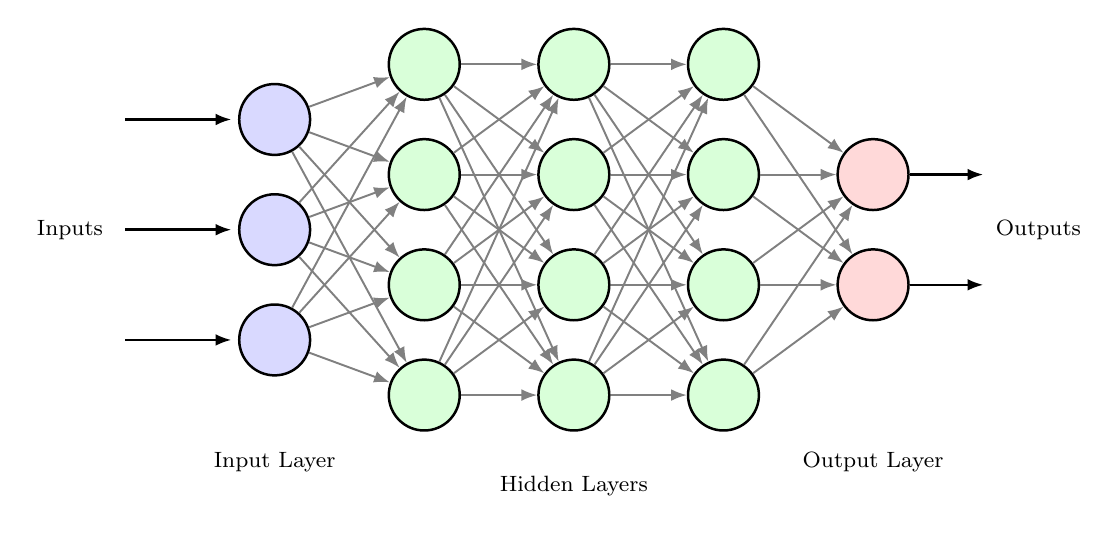
\begin{tikzpicture}[
    neuron/.style={
        circle,
        draw=black,
        line width=0.9pt,
        minimum size=9mm
    },
    input neuron/.style={
        neuron,
        fill=blue!15
    },
    hidden neuron/.style={
        neuron,
        fill=green!15
    },
    output neuron/.style={
        neuron,
        fill=red!15
    },
    conn/.style={
        -{Latex[length=2mm]},
        draw=gray!100,
        line width=0.7pt
    },
    io/.style={
        -{Latex[length=2mm]},
        draw=black,
        line width=0.9pt
    },
    label/.style={
        font=\footnotesize,
        text=black
    }
]

% ------------------------------------------------
% Input arrows
% ------------------------------------------------
\draw[io] (-0.9,  1.4) -- (0.45,  1.4);
\draw[io] (-0.9,  0.0) -- (0.45,  0.0);
\draw[io] (-0.9, -1.4) -- (0.45, -1.4);

\node[label] at (-1.6,0) {Inputs};

% ------------------------------------------------
% Input layer
% ------------------------------------------------
\node[input neuron]  (I1) at (1.0,  1.4) {};
\node[input neuron]  (I2) at (1.0,  0.0) {};
\node[input neuron]  (I3) at (1.0, -1.4) {};

% ------------------------------------------------
% Hidden layer 1
% ------------------------------------------------
\node[hidden neuron] (H11) at (2.9,  2.1) {};
\node[hidden neuron] (H12) at (2.9,  0.7) {};
\node[hidden neuron] (H13) at (2.9, -0.7) {};
\node[hidden neuron] (H14) at (2.9, -2.1) {};

% ------------------------------------------------
% Hidden layer 2
% ------------------------------------------------
\node[hidden neuron] (H21) at (4.8,  2.1) {};
\node[hidden neuron] (H22) at (4.8,  0.7) {};
\node[hidden neuron] (H23) at (4.8, -0.7) {};
\node[hidden neuron] (H24) at (4.8, -2.1) {};

% ------------------------------------------------
% Hidden layer 3
% ------------------------------------------------
\node[hidden neuron] (H31) at (6.7,  2.1) {};
\node[hidden neuron] (H32) at (6.7,  0.7) {};
\node[hidden neuron] (H33) at (6.7, -0.7) {};
\node[hidden neuron] (H34) at (6.7, -2.1) {};

% ------------------------------------------------
% Output layer
% ------------------------------------------------
\node[output neuron] (O1) at (8.6,  0.7) {};
\node[output neuron] (O2) at (8.6, -0.7) {};

% ------------------------------------------------
% Connections: input -> hidden 1
% ------------------------------------------------
\foreach \i in {I1,I2,I3}
    \foreach \j in {H11,H12,H13,H14}
        \draw[conn] (\i) -- (\j);

% Hidden 1 -> hidden 2
\foreach \i in {H11,H12,H13,H14}
    \foreach \j in {H21,H22,H23,H24}
        \draw[conn] (\i) -- (\j);

% Hidden 2 -> hidden 3
\foreach \i in {H21,H22,H23,H24}
    \foreach \j in {H31,H32,H33,H34}
        \draw[conn] (\i) -- (\j);

% Hidden 3 -> output
\foreach \i in {H31,H32,H33,H34}
    \foreach \j in {O1,O2}
        \draw[conn] (\i) -- (\j);

% ------------------------------------------------
% Output arrows
% ------------------------------------------------
\draw[io] (O1) -- (10.0,  0.7);
\draw[io] (O2) -- (10.0, -0.7);

\node[label] at (10.7,0) {Outputs};

% ------------------------------------------------
% Layer labels
% ------------------------------------------------
\node[label] at (1.0,-2.95) {Input Layer};
\node[label] at (4.8,-3.25) {Hidden Layers};
\node[label] at (8.6,-2.95) {Output Layer};

\end{tikzpicture}
%
    }
    \caption{Fully-connected feed-forward network: input layer, three hidden
    layers, and output layer.  The actor and critic in this work use separate
    \glspl{mlp} of this form.}
    \label{fig:mlp}
\end{figure}

Network parameters are collected into a vector $\theta$ and optimized by
minimizing a loss function $\mathcal{L}(\theta)$ via stochastic gradient
descent or one of its adaptive variants (Adam, RMSProp).  The gradient
$\nabla_\theta \mathcal{L}$ is computed efficiently by
\emph{backpropagation}, which applies the chain rule layer by layer from the
output back to the inputs~\cite{goodfellow2016deep}.  In the RL setting
discussed in Section~\ref{sec:rl}, the loss is derived from the policy
objective $J(\theta)$ and the critic's value-prediction error, so the same
backpropagation machinery drives both the actor and critic updates.

\subsection{Deep Learning}

\emph{Deep learning} refers to the use of neural networks with many hidden
layers.  Greater depth allows the network to compose simple transformations
into increasingly abstract representations: early layers typically capture
low-level features while later layers encode task-relevant structure.  This
hierarchical inductive bias has proven effective across perception, language,
and control, including in high-dimensional continuous-control settings
directly comparable to this work~\cite{silver2016mastering,berner2019dota}.

For the \gls{vsss} policy, the observation vector includes the positions,
orientations, and velocities of all robots and the ball — the full simulator
state — so no hidden dynamics need to be inferred from a history of frames.
Recurrent architectures are therefore unnecessary; a feed-forward network
suffices.  A fully-connected
\gls{mlp} with two or three hidden layers captures the required nonlinear
dependencies while remaining fast to evaluate on a \gls{gpu} across thousands
of parallel environments.  The actor and critic each use a separate
\gls{mlp}; sharing lower layers is possible but not assumed in the baseline
design.

Two practical techniques are relevant to stability in deep \gls{rl}.  First,
layer normalization~\cite{goodfellow2016deep} standardizes activations within
each layer, reducing sensitivity to the scale of inputs and mitigating the
non-stationarity of the input distribution that arises because the policy
changes throughout training.  Second, the outputs of the final actor layer
are initialized with small weights so that the policy starts close to a
uniform distribution, allowing the agent to explore broadly early in
training.  Both choices are standard in the \gls{ppo} implementations applied
to continuous-control domains.

\section{Reinforcement Learning}
\label{sec:rl}

\subsection{Fundamentals}

Reinforcement learning formalizes sequential decision-making as interaction
between an agent and an environment~\cite{sutton2018reinforcement}.  In the
Markov decision process (\gls{mdp}) formulation, the environment is described
by the tuple $\langle \mathcal{S}, \mathcal{A}, \mathcal{P}, R, \gamma
\rangle$, where $\mathcal{S}$ is the state space, $\mathcal{A}$ is the action
space, $\mathcal{P}(s_{t+1} \mid s_t, a_t)$ is the transition distribution,
$R$ is the reward function, and $\gamma \in [0,1]$ is the discount factor.

The agent acts according to a policy $\pi_\theta$ parameterized by $\theta$.
Its objective is to maximize the expected discounted return:
%
\begin{equation}
    J(\theta) = \mathbb{E}_{\pi_\theta}\!\left[\sum_{t=0}^{T} \gamma^t
    r_t\right].
\end{equation}
%
Value functions summarize long-term quality.  The state-value function
$V^\pi(s)$ gives the expected return from state $s$ under $\pi$, and the
action-value function $Q^\pi(s,a)$ conditions additionally on taking action
$a$.  The advantage function,
%
\begin{equation}
    A^\pi(s,a) = Q^\pi(s,a) - V^\pi(s),
\end{equation}
%
measures how much better or worse a particular action is relative to the
policy's average behavior in that state.  This quantity appears centrally in
the policy-gradient and actor-critic methods described below.

\subsection{Policy Gradient, Actor-Critic, and PPO}

Policy-gradient methods optimize $\pi_\theta$ directly via gradient ascent on
$J(\theta)$.  The standard estimator is
%
\begin{equation}
    \nabla_\theta J(\theta) =
    \mathbb{E}\!\left[
        \nabla_\theta \log \pi_\theta(a_t \mid s_t)\,\hat{A}_t
    \right],
    \label{eq:pg}
\end{equation}
%
where $\hat{A}_t$ is a sampled estimate of the advantage.  The estimator is
unbiased but can exhibit high variance, which makes learning slow or unstable.
Actor-critic methods reduce this variance by learning a parametric critic
$V_w(s)$ alongside the policy.  The critic supplies the baseline needed to
compute $\hat{A}_t$ via Generalized Advantage Estimation
(GAE)~\cite{schulman2015gae}:
%
\begin{equation}
    \hat{A}_t^{\mathrm{GAE}} = \sum_{k=0}^{T-t}(\gamma\lambda)^k\,\delta_{t+k},
    \qquad
    \delta_t = r_t + \gamma V_w(s_{t+1}) - V_w(s_t),
    \label{eq:gae}
\end{equation}
%
where $\lambda \in [0,1]$ trades variance against bias: $\lambda \to 0$
relies heavily on the critic estimate, and $\lambda \to 1$ relies more on
actual returns.

\gls{ppo}~\cite{schulman2017ppo} extends the actor-critic framework with a
constraint that prevents destructively large policy updates.  It defines the
probability ratio $r_t(\theta) = \pi_\theta(a_t \mid s_t) /
\pi_{\theta_\mathrm{old}}(a_t \mid s_t)$ and optimizes the clipped surrogate
objective:
%
\begin{equation}
    L^{\mathrm{CLIP}}(\theta) =
    \mathbb{E}\!\left[
        \min\!\left(
            r_t(\theta)\,\hat{A}_t,\;
            \mathrm{clip}\!\left(r_t(\theta),\,1-\varepsilon,\,1+\varepsilon\right)
            \hat{A}_t
        \right)
    \right].
    \label{eq:ppo}
\end{equation}
%
The clipping parameter $\varepsilon$ bounds how far $\pi_\theta$ may deviate
from the behavior policy that collected the data, removing the incentive to
take excessively large gradient steps.  Because a single batch can be reused
for several gradient epochs before being discarded, \gls{ppo} achieves better
sample efficiency than a plain policy-gradient update while remaining simpler
to implement than \gls{trpo}~\cite{schulman2015trpo}.


Its robustness across the \gls{vsss} domain~\cite{tg_thiago,tg_thay,brandao2022} make it the
natural algorithm choice for this work.

% ------------------------------------------------------------------
\subsection{Curriculum Learning}
% ------------------------------------------------------------------

Curriculum learning organizes the training process as a sequence of tasks of
increasing difficulty, rather than exposing the agent to the final task from
the start~\cite{bengio2009curriculum}.  The motivation is practical: in
settings with sparse rewards or a large initial performance gap between random
and competent behavior, a policy initialized at random may never encounter
enough informative signal to make progress.  A curriculum provides a ramp that
keeps the task at a difficulty where learning can occur.

For \gls{vsss}, the final objective — winning 3v3 matches — is far too complex
for a randomly-initialized policy to explore productively.  A staged approach
addresses this: allied robots first practice ball conduction and basic
positioning without any opposition, then face opponents only once those
sub-skills are established.

% ------------------------------------------------------------------
\subsection{Prioritized Level Replay}
% ------------------------------------------------------------------

\gls{plr}~\cite{prioritized_level_replay} is a mechanism for allocating training
experience across a distribution of situations, or \emph{levels}, according to
an estimate of their future learning potential rather than uniformly at random.
The core observation is that, at any point in training, some situations will
be either too easy (the agent already solves them reliably) or too hard
(the agent cannot yet extract any useful gradient).  The most informative
situations are those at the boundary of current competence.

After each episode on level $l_i$, \gls{plr} computes a score
%
\begin{equation}
    S_i = \frac{1}{T}\sum_{t=0}^{T}\bigl|\hat{A}_t^{\mathrm{GAE}}\bigr|,
    \label{eq:plr_score}
\end{equation}
%
the mean absolute \gls{gae} over the trajectory~\cite{prioritized_level_replay}.  This
quantity is equivalent to the mean $L_1$ value loss under \gls{ppo}, and
levels on which the critic is most surprised carry the highest priority.  A
staleness correction down-weights levels that have not been visited recently,
preventing the replay distribution from becoming stale with respect to a
policy that has since improved.  The resulting sampling distribution
$P_{\mathrm{replay}}$ interpolates between high-priority (high value-error)
and unseen levels, inducing an implicit curriculum without requiring prior
knowledge of level difficulty.

In the context of this thesis, a level is a game initialization: robot poses,
ball position, velocities, and any relevant game-state context.  Because
\gls{vsss} admits a large space of initial configurations with very unequal
learning value, \gls{plr} is a natural fit.  The high-throughput simulator
developed here makes the approach practical: with enough parallel environments,
the overhead of maintaining a priority buffer and replaying specific
initializations is negligible compared to the benefit of directing more
experience toward informative situations.

% ------------------------------------------------------------------
\subsection{Multi-Agent Reinforcement Learning and Self-Play}
% ------------------------------------------------------------------

When several policies act in the same environment, the standard single-agent
\gls{mdp} formulation no longer fully characterizes the learning problem.  Each
agent's optimal policy depends on the behavior of the others, which themselves
change during training — a property known as non-stationarity.  In cooperative
settings this manifests as a credit-assignment problem: individual contributions
to a shared reward are difficult to attribute.  In competitive settings, the
moving target created by an improving opponent can destabilize learning.  Robot
soccer combines both regimes within the same episode.

Self-play addresses the competitive aspect by using the agent itself — or
previously saved versions — as the opponent.  The opponent automatically
becomes harder as the agent improves, creating a natural difficulty curriculum.
However, training exclusively against the latest version of the policy can lead
to \emph{strategy collapse}: the agent discovers a local best-response that
dominates the current opponent but is easily exploited by a broader range of
strategies.  Fictitious self-play~\cite{brown1951fsp} mitigates this by playing
against a mixture over all historical policies, with convergence guarantees for
two-player zero-sum games.  In practice, emphasizing more recent opponents
while retaining some probability on older ones achieves a good balance between
generalization and training efficiency — the family of opponent-sampling
schemes studied by \cite{master_thay} and the league-training approach of
\cite{starcraft_marl} are both instances of this principle.

\gls{ctde} is a standard architecture for cooperative teams: during training,
each agent's critic may access global state to produce more accurate value
estimates, while the policies themselves are conditioned only on locally
available observations.  At execution time the critics are discarded, and each
robot acts from its own observation alone.  This separation allows the critic
to leverage information that would not be available in deployment without
constraining the policy to require it.

% ------------------------------------------------------------------
\subsection{Exploiting Symmetry in the VSSS Problem}
% ------------------------------------------------------------------

The 3v3 \gls{vsss} setting has two classes of symmetry that can be exploited
to improve learning efficiency.

\textbf{Permutation symmetry.}  The three robots on the same team are
homogeneous: they have identical kinematics and contribute to the same team
objective.  The value of a team state should therefore be invariant to which
robot is labeled 1, 2, or 3.  Sharing policy and critic parameters across all
three robots exploits this directly — a single network is updated using
transitions from all three agents simultaneously, tripling effective data
throughput without requiring a larger batch.  \textcite{brandao2022} applied
exactly this principle in their \gls{vsss} multi-agent formulation, observing
that shared parameters provide a natural implicit regularization.

\textbf{Reflection symmetry.}  The VSSS field is bilaterally symmetric about
its longitudinal axis.  A game state mirrored across that axis, with signs of
transverse coordinates flipped consistently for positions, velocities, and
actions, is an equally valid game state with the same value.  This symmetry
can be exploited through data augmentation: every collected transition generates
a second, reflected transition at no additional simulation cost, doubling the
effective number of distinct states the policy is trained on.

Both forms of symmetry are treated as first-class design choices in the
training methodology rather than as optional post-processing.

% ------------------------------------------------------------------
\section{High-Throughput, GPU-Accelerated Simulation}
% ------------------------------------------------------------------

On-policy algorithms like \gls{ppo} repeatedly collect fresh rollouts and
discard them after a single round of updates.  The number of environment steps
per wall-clock second is therefore a direct multiplier on how much training
progress can be made in a given time budget.  When the simulator is the
bottleneck, improvements to the learning algorithm yield diminishing returns.

\gls{jax}~\cite{jax2018github} provides three complementary transformations
that make GPU-parallel simulation practical.  \texttt{jit} compiles a
numerical function to native code, eliminating Python overhead.  \texttt{vmap}
lifts a single-environment step into a vectorized step over a batch of
environments, enabling thousands of independent games to advance in a single
device call.  \texttt{scan} implements a fixed-length loop (a rollout horizon)
as a single compiled operation, avoiding repeated Python-level dispatch.
Because \gls{jax} programs are purely functional, state is passed explicitly
with no hidden side-effects, so the entire collect-and-update loop runs on the
accelerator without data copies between host and device.

For \gls{vsss}, the physics model — rigid-body kinematics, elastic wall
collisions, and a friction model for ball--floor contact — is simple enough
to implement as differentiable array operations without any approximation that
would matter for policy learning.

\chapter{Methodology}
% ============================================================
%  CHAPTER 4 — METHODOLOGY (PROPOSAL)
%
%  Proposed reorganization (simulator-first, then RL, PLR last):
%
%   4.1  Overview                          (NEW — orients the reader)
%   4.2  The High-Throughput GPU Simulator (the enabling artifact)
%        4.2.1 Simulator state and step interface
%        4.2.2 Physics model
%        4.2.3 Batching and rollout collection
%   4.3  Problem Formulation               (centralized-joint-control MDP)
%        4.3.1 State and observation space
%        4.3.2 Action space
%        4.3.3 Reward function
%        4.3.4 Transition and discount
%   4.4  Policy Architecture               (centralized joint controller; CTDE deferred to TG-2)
%   4.5  Exploiting Symmetries
%   4.6  Two-Stage Curriculum and Self-Play
%   4.7  Prioritized-Level-Replay Sampler  (second contribution, own section)
%   4.8  Tooling and Infrastructure
%   4.9  Scope and Discarded Alternatives  (already written — keep at end)
%
%  Rationale: the simulator is the enabling artifact, so it comes first.
%  The MDP formulation then describes WHAT is being learned on top of it.
%  PLR is pulled out into its own section (not buried among RL details)
%  because it is the planned sample-selection mechanism for TG-2.
% ============================================================

This chapter defines the proposed methodology.  It begins with the
high-throughput simulator, the enabling artifact on which everything else
depends, then formulates the 3v3 task as a multi-agent reinforcement-learning
problem, describes the policy architecture and the mechanisms that exploit the
domain's symmetries, and presents the two-stage curriculum and
prioritized-level-replay sampler interface.  The chapter closes with the
tooling and a statement of scope.

% ==================================================================
\section{Overview}
% ==================================================================

The methodology realizes the two contributions of
Section~\ref{sec:contributions} within a common training loop: the simulator
generates batched rollouts, a \gls{ppo} learner consumes them, and the
initialization mechanism determines which situations to sample next.  The
remaining sections specify each component.

% ============================================================
%  TG-1 training-infrastructure diagram (revised).
%
%  Structural changes from the initial version:
%   – Learner and Policy merged into one SB3 PPO box.
%     The standard SB3 OnPolicyAlgorithm is a single synchronous
%     process; a two-box design implied an actor–learner split
%     (e.g. IMPALA) that does not exist in TG-1.
%   – JAX↔PyTorch device boundary made the visual focal point,
%     matching the throughput argument in Chapter 5.
%     All per-step obs/act data crosses this line every step.
%   – Opponent team explicitly shown in Environments.
%   – "On-device training loop" container removed: it spanned
%     both the JAX device and the PyTorch/CPU learner, making
%     "on-device" self-contradictory.
%
%  Required preamble (already present in tese.tex):
%      \usepackage{tikz}
%      \usetikzlibrary{arrows.meta,shapes,positioning}
% ============================================================

% ---- palette ----
\definecolor{tgDeepBlue}{RGB}{17,52,160}
\definecolor{tgTileBlue}{RGB}{96,141,224}
\definecolor{tgPaleBlue}{RGB}{223,231,249}
\definecolor{tgGold}{RGB}{245,199,38}
\definecolor{tgPaleGold}{RGB}{253,243,205}
\definecolor{tgCrimson}{RGB}{214,40,87}
\definecolor{tgArrow}{RGB}{40,40,55}

% ---- centred grid of small tiles (drawn from current origin) ----
% #1=lastCol (cols-1)  #2=lastRow (rows-1)  #3=colour  #4=step  #5=cell
\providecommand{\tgtiles}[5]{%
  \foreach \tx in {0,...,#1}{%
    \foreach \ty in {0,...,#2}{%
      \fill[#3] (\tx*#4 - #1*#4/2 - #5/2, \ty*#4 - #2*#4/2 - #5/2)
                rectangle +(#5,#5);}}%
}

\begin{figure}[ht]
    \centering
    \resizebox{\textwidth}{!}{%
    \begin{tikzpicture}[
        font=\scriptsize,
        card/.style={draw=tgDeepBlue, line width=0.8pt, rounded corners=2pt},
        flow/.style={-{Latex[length=2.2mm,width=1.8mm]}, line width=0.9pt, draw=tgArrow},
        lab/.style={font=\scriptsize, text=tgArrow, fill=white, inner sep=1.2pt},
        sub/.style={font=\tiny, align=center, text=tgDeepBlue!85!black},
    ]

    % ===== Background tints: CPU side (left) vs JAX side (right) =============
    % White strip at x=7.3–7.7 keeps the boundary line visually clear.
    \fill[tgPaleGold!30] (-0.2,-2.3) rectangle (7.3,5.7);
    \fill[tgPaleBlue!30] (7.7,-2.3) rectangle (15.2,5.7);

    % ===== JAX ↔ PyTorch device boundary — visual focal point ================
    \draw[line width=1.5pt, draw=tgCrimson] (7.5,-2.3) -- (7.5,5.7);
    \node[fill=white, text=tgCrimson, font=\tiny\bfseries,
          inner sep=2pt, align=center]
        at (7.5,5.5) {device\,$\leftrightarrow$\,host\\[-1pt](per-step)};

    % ===== Side labels =======================================================
    \node[font=\tiny\itshape, text=tgDeepBlue!70]
        at (3.0,-2.15) {CPU / PyTorch (host)};
    \node[font=\tiny\itshape, text=tgDeepBlue!70]
        at (12.2,-2.15) {JAX accelerator (device)};

    % ========================= SB3 PPO card (CPU side) =======================
    \node[card, fill=tgPaleGold, minimum width=5.2cm, minimum height=3.0cm]
        (sb3) at (3.0,0) {};
    \begin{scope}
      \clip[rounded corners=2pt] (sb3.south west) rectangle (sb3.north east);
      \fill[tgDeepBlue] ([yshift=-0.5cm]sb3.north west) rectangle (sb3.north east);
    \end{scope}
    \node[white, font=\scriptsize\bfseries]
        at ([yshift=-0.25cm]sb3.north) {SB3 PPO (PyTorch $\cdot$ CPU)};
    \begin{scope}[shift={(3.0,0.15)}]
        \tgtiles{3}{2}{tgGold}{0.26}{0.18}
    \end{scope}
    \node[sub] at (3.0,-0.82)
        {MLP $\pi_\theta$ (actor+critic trunk)\\
         single-process \texttt{OnPolicyAlgorithm}\\
         PPO gradient updates};

    % ========================= ENVIRONMENTS card (JAX side) ==================
    \node[card, fill=tgPaleBlue, minimum width=5.2cm, minimum height=3.0cm]
        (env) at (12.2,0) {};
    \begin{scope}
      \clip[rounded corners=2pt] (env.south west) rectangle (env.north east);
      \fill[tgDeepBlue] ([yshift=-0.5cm]env.north west) rectangle (env.north east);
    \end{scope}
    \node[white, font=\scriptsize\bfseries]
        at ([yshift=-0.25cm]env.north) {Environments};
    \begin{scope}[shift={(12.2,0.15)}]
        \tgtiles{5}{3}{tgTileBlue}{0.22}{0.15}
    \end{scope}
    \node[sub] at (12.2,-0.82)
        {\texttt{VSSVecEnv} $\cdot$ JAX $\cdot$
         $\mathrm{jit}(\mathrm{vmap}(\texttt{step}))$\\
         256--1024 parallel matches\\
         opponent: scripted / frozen $\pi^{(t-k)}_\theta$};

    % ============================ MLflow card ================================
    \node[card, fill=tgPaleBlue, minimum width=3.8cm, minimum height=1.55cm]
        (mlflow) at (3.0,4.4) {};
    \begin{scope}
      \clip[rounded corners=2pt] (mlflow.south west) rectangle (mlflow.north east);
      \fill[tgDeepBlue] ([yshift=-0.42cm]mlflow.north west) rectangle (mlflow.north east);
    \end{scope}
    \node[white, font=\scriptsize\bfseries]
        at ([yshift=-0.21cm]mlflow.north) {MLflow tracking};
    \begin{scope}[shift={(3.0,4.55)}]
        \tgtiles{4}{1}{tgTileBlue}{0.2}{0.13}
    \end{scope}
    \node[sub] at (3.0,4.12)
        {reward (mean/min) $\cdot$ ep.\ length\\throughput $\cdot$ checkpoints};

    % ========================= INITIALIZATION card ===========================
    \node[card, fill=tgPaleBlue, minimum width=4.2cm, minimum height=1.55cm]
        (init) at (12.2,4.4) {};
    \begin{scope}
      \clip[rounded corners=2pt] (init.south west) rectangle (init.north east);
      \fill[tgDeepBlue] ([yshift=-0.42cm]init.north west) rectangle (init.north east);
    \end{scope}
    \node[white, font=\scriptsize\bfseries]
        at ([yshift=-0.21cm]init.north) {Initialization};
    \begin{scope}[shift={(12.2,4.55)}]
        \tgtiles{4}{1}{tgTileBlue}{0.2}{0.13}
    \end{scope}
    \node[sub] at (12.2,4.12)
        {\texttt{InitMode}: kickoff / random\\($\rightarrow$ PLR sampler, TG-2)};

    % ============================ ARROWS =====================================

    % Per-step: allied action SB3 → Env (crosses device boundary)
    \draw[flow] ([yshift=0.5cm]sb3.east) -- ([yshift=0.5cm]env.west)
        node[lab, pos=0.25] {act $a\!\in\!\mathbb{R}^{6}$ (allied)};
    % Per-step: observation Env → SB3 (crosses device boundary)
    \draw[flow] ([yshift=-0.5cm]env.west) -- ([yshift=-0.5cm]sb3.east)
        node[lab, pos=0.75] {obs $o\!\in\!\mathbb{R}^{46}$};

    % Gymnasium ⇌ SB3 adapter sitting ON the boundary —
    % mediates every per-step obs/act transfer
    \node[draw=tgDeepBlue, line width=0.8pt, fill=white, rounded corners=2pt,
          align=center, font=\tiny, inner sep=2.5pt]
        at (7.5,0) {Gymnasium\,$\rightleftarrows$\,SB3\\adapter};

    % Rollout buffer returned after N steps (bottom path)
    \draw[flow] (env.south) -- (12.2,-1.85) -- (3.0,-1.85) -- (sb3.south);
    \node[lab] at (7.5,-1.85)
        {rollout $(o,a,r,\text{done})$ — $N$ steps};

    % Initialization → Environments
    \draw[flow] (init.south) -- (env.north)
        node[lab, midway] {initial states};

    % SB3 → MLflow
    \draw[flow] (sb3.north) -- (mlflow.south)
        node[lab, midway] {metrics};

    \end{tikzpicture}%
    }
    \caption{Training infrastructure for the TG-1 smoke tests
    (\texttt{scripts/smoke.py}).  The figure is organised around the
    \textbf{device\,$\leftrightarrow$\,host boundary} (red vertical line):
    the CPU/PyTorch side (left, warm tint) holds the PPO learner, and the
    JAX accelerator side (right, blue tint) holds the vectorised
    environments.  \emph{Every step}, the environment receives the allied
    action $a\!\in\!\mathbb{R}^{6}$ (wheel speeds for all three robots
    output by the centralized MLP $\pi_\theta$) and an opponent action
    (scripted agent or frozen checkpoint $\pi^{(t-k)}_\theta$), then
    returns observation $o\!\in\!\mathbb{R}^{46}$ (positions, velocities,
    and headings of all six robots plus the ball).  Both arrays must cross
    the Gymnasium\,$\rightleftarrows$\,SB3 adapter on every call
    (device$\to$host for obs; host$\to$device for act); this per-step
    transfer is the throughput bottleneck motivating the JAX-native
    training loop planned for TG-2.  The \textbf{SB3 PPO box is a single
    synchronous process} (\texttt{OnPolicyAlgorithm}): there is no
    actor--learner split; \texttt{collect\_rollouts} and \texttt{train}
    share the same MLP object (actor and critic share an MLP trunk ---
    not per-agent parameter sharing); the learner is intentionally placed
    on CPU to avoid GPU contention with the JAX device.  After $N$ steps
    the accumulated rollout buffer feeds the PPO update.  Episode resets
    use the pluggable \texttt{InitMode} (the future PLR sampler insertion
    point), and MLflow logs per-episode mean/min reward, episode length,
    throughput, and checkpoints.  The centralized joint-control
    formulation (one MLP, one team) is the TG-1 baseline;
    per-agent parameter sharing and \gls{ctde} are deferred to TG-2.}
    \label{fig:training_infra}
\end{figure}



% ==================================================================
\section{The High-Throughput GPU Simulator}
% ==================================================================

The simulator is implemented as a pure, batched JAX environment, designed for
speed, numerical stability, and full on-accelerator execution so that the
entire collect-and-update loop runs without per-step transfers to host memory.

% ------------------------------------------------------------------
\subsection{Simulator State and Step Interface}
% ------------------------------------------------------------------

A simulator state stores the poses and velocities of the six robots, the
position and velocity of the ball, the score, episode timers, and the
pseudo-random generator keys.  In the JAX backend this state is an immutable
\texttt{NamedTuple} PyTree, which makes it directly compatible with
\texttt{jax.vmap} batching.  The environment exposes two functions:
%
\begin{itemize}
    \item \texttt{reset(key)} initializes one or more game states according to
    the selected initialization mode;
    \item \texttt{step(state, action)} advances the physics by one timestep and
    returns the next state together with observations, rewards, termination
    flags, and diagnostic information.
\end{itemize}

% ------------------------------------------------------------------
\subsection{Physics Model}
\label{sec:physics_model}
% ------------------------------------------------------------------

The physics model is two-dimensional and captures the interactions that shape
policy learning: differential-drive motion, ball dynamics under friction,
robot–ball and robot–robot contact, and wall and goal handling on an IEEE VSSS
field.  Numeric dimensions (field size, robot footprint, ball diameter, goal
opening, wheelbase, and control rate) follow the competition specification and
are centralized in the implementation configuration module
(\texttt{vsss\_sim.config}).  The subsections below state \emph{why} each
modelling choice was made; run-specific training overrides are reported
separately in Chapter~5 (Table~\ref{tab:smoke_config}).

\subsubsection{Scope and fidelity}
\label{sec:physics_scope}

TG-1 prioritizes a simulator that is fast, batched, and stable enough for
large-scale \gls{ppo} rollouts over reproducing every effect of the team's
legacy C++/ODE stack.  The model is planar: no vertical dynamics,
no wheel slip model, and no explicit motor controller beyond rate-limited wheel
commands.  That scope matches the scale of Very Small Size Soccer, where the
dominant learning signal comes from ball interaction and team positioning
rather than from high-fidelity drivetrain modeling.

\subsubsection{Geometry, coordinates, and goals}

The regulation field layout is Figure~\ref{fig:field} (Chapter~2).  In the
simulator the origin is at the field centre, $+x$ points toward the opponent
goal, and $+y$ is parallel to the goal line (Section~\ref{sec:ma_coords}).
Each team fields three robots as $7.5 \times 7.5$\,cm \textbf{oriented bounding
boxes (OBBs)} with circle--OBB ball contact (not circular robot proxies).
Goals are $40$\,cm openings; scoring triggers an in-episode kickoff, not a
terminal state.

\subsubsection{Time stepping and actuation}

Control commands arrive at $60$\,Hz ($\Delta t = 1/60$\,s).  Each control step
is subdivided into \textbf{four physics sub-steps} (\texttt{SUB\_STEPS}), so
collisions and ball motion are integrated at $240$\,Hz effective resolution
without increasing the policy's decision frequency.  Robots are
\textbf{differential-drive}: normalized actions in $[-1,1]$ map to left and
right wheel speeds, then to body-frame $(v_x, v_y, \omega)$ via the standard
kinematic relation with wheelbase $53$\,mm and maximum linear speed
$\sim 1.30$\,m/s.

Wheel speeds do not jump instantaneously to the commanded value.  Each sub-step
limits the change in wheel speed to approximate motor slew (\texttt{ROBOT\_WHEEL\_ACCEL\_LIMIT} $\approx 1\,g$), which smooths trajectories and avoids
unphysically sharp turns that would otherwise appear when a neural policy
outputs discontinuous commands.  Heading is wrapped to $(-\pi, \pi]$ after
integration.

\subsubsection{Contact dynamics and ball motion}

Between commands, the ball experiences rolling friction (coefficient
\texttt{BALL\_FRICTION}) and elastic-style impulses on walls and robots
(restititution parameters in \texttt{config}).  Robot–wall contact clamps the
OBB inside the field and zeroes velocity components that point into the wall.
Robot–robot collisions use separating axes on the square footprints with
impulse exchange.  These rules are hand-tuned for stable, non-exploding
contacts at VSSS speeds rather than for exact material parameters; the goal is
repeatable interaction statistics for learning, not a calibrated multibody
model.

\subsubsection{Physics design choices}
\label{sec:physics_design}

Table~\ref{tab:physics_design} summarizes the main modelling decisions and
their rationale.  Together they define the physics contract that both backends
implement.

\begin{table}[ht]
    \centering
    \caption{Physics design choices in the VSSS simulator.
    Numeric constants live in \texttt{vsss\_sim.config}.}
    \label{tab:physics_design}
    \small
    \begin{tabular}{p{0.22\linewidth}p{0.38\linewidth}p{0.34\linewidth}}
        \toprule
        \textbf{Choice} & \textbf{Mechanism} & \textbf{Rationale} \\
        \midrule
        Planar 2D engine &
        State: ball $(x,y,v_x,v_y)$; robots $(x,y,\theta,v_x,v_y,\omega)$ &
        Matches top-down VSSS; enables batched array physics. \\
        \addlinespace
        OBB robots &
        Square footprint; circle–OBB for ball; SAT for robot–robot &
        Avoids disk proxy errors at $7.5$\,cm scale. \\
        \addlinespace
        Sub-stepped integration &
        $4\times$ substeps per $60$\,Hz control step &
        Reduces tunneling and stabilizes contacts at max wheel speed. \\
        \addlinespace
        Rate-limited wheels &
        Slew cap $\approx 1\,g$ per sub-step on each wheel &
        Models torque limits; smoother policy rollouts. \\
        \addlinespace
        Differential drive &
        Wheel speeds $\rightarrow$ $(v,\omega)$ $\rightarrow$ world velocity &
        Matches IEEE VSS hardware; action space is six wheel commands. \\
        \addlinespace
        Rolling ball friction &
        Deceleration $\propto \mu_r g \,\Delta t_{\mathrm{sub}}$ &
        Ball comes to rest without explicit spin state. \\
        \addlinespace
        Restitution on impact &
        Separate coeffs.\ for ball–wall, ball–robot, robot–wall &
        Tunable bounce; prevents energy blow-up in dense clusters. \\
        \addlinespace
        Goals without terminal &
        Score event + kickoff reset; episode ends on step cap only &
        Aligns with continuous play; keeps \texttt{terminated}$=$\texttt{False}. \\
        \bottomrule
    \end{tabular}
\end{table}

% ------------------------------------------------------------------
\subsection{Batching and Rollout Collection}
% ------------------------------------------------------------------

The environment is vectorized across many parallel games by applying
$\mathrm{jit}(\mathrm{vmap}(\texttt{step}))$ to a single batched state, so that
one compiled call advances an entire batch of independent matches.  Rollouts for
\gls{ppo} are collected by scanning the step function through time and mapping
it across environments, keeping trajectory buffers resident on the device.

%% FIGURE: on-device training loop — batched SimState → jit(vmap(step)) →
%% observations/rewards → PPO update → next initial states (from the sampler).
%% Place beside the Chapter 2 socket-loop figure so the architectural shift is
%% visible; both should be your own diagrams in a consistent visual style.

% ==================================================================
\section{Problem Formulation}
% ==================================================================

The 3v3 \gls{vsss} task is the domain within which both contributions are
evaluated.  In TG-1, the team is controlled by a \textbf{centralized joint
policy}: a single network observes the full global state of all six robots and
the ball ($\mathbb{R}^{46}$) and outputs a joint action that simultaneously
commands all three allied robots ($\mathbb{R}^{6}$).  Although the domain is
inherently multi-agent, this centralized formulation treats the three-robot
team as a single composite agent, which simplifies the implementation and
provides a clean baseline.  The observation interface is factored as a
swappable function, so the per-robot egocentric formulation required by
\gls{ctde} can be adopted without changes to the simulator.  This section
defines the components of the underlying decision process: state and
observation space, action space, reward, and transition dynamics.

\label{sec:ma_coords}
The learning frame uses the centred simulator coordinates of
Figure~\ref{fig:field}: origin at field centre, $+x$ toward the opponent goal,
$+y$ along the goal line.

% ------------------------------------------------------------------
\subsection{State and Observation Space}
% ------------------------------------------------------------------

The full simulator state is described in Section~4.2.  From it, the learning
system builds a per-step observation vector of dimension 46, composed of the
ball state and the state of all six robots, normalized so that equivalent
situations have similar numerical representations.  The ball contributes its
position and velocity; each robot contributes its position, orientation, and
linear and angular velocity.  Orientation is encoded as the pair
$(\sin\theta, \cos\theta)$ rather than the raw angle, to avoid the
discontinuity at $\pm\pi$ and to give the network a smooth representation of
heading.  Table~\ref{tab:obs} summarizes the observation layout and the
normalization applied to each group.

\begin{table}[ht]
    \centering
    \caption{Observation vector ($\mathbb{R}^{46}$) layout and normalization.
    Positions are normalized by the half-field dimensions, linear velocities by
    $1.5\times$ the maximum wheel speed, and angular velocity by the maximum
    achievable rate implied by the wheelbase.}
    \label{tab:obs}
    \begin{tabular}{lll}
        \toprule
        \textbf{Indices} & \textbf{Content} & \textbf{Per element} \\
        \midrule
        $[0\!:\!4]$  & ball               & $x, y, v_x, v_y$ (normalized) \\
        $[4\!:\!46]$ & 6 robots $\times$ 7 & $x, y, \sin\theta, \cos\theta, v_x, v_y, \omega$ \\
        \bottomrule
    \end{tabular}
\end{table}

The observation construction is factored as a swappable function.  This keeps
the interface forward-compatible with per-robot egocentric observations, which
the multi-agent variants planned for TG-2 require, without changing the
simulator.

% ------------------------------------------------------------------
\subsection{Action Space}
% ------------------------------------------------------------------

The action space is continuous.  In the baseline formulation, the policy
controls all three allied robots through a single 6-dimensional action — a
normalized left/right wheel-speed pair per robot, in $[-1, 1]$ — which is
denormalized to physical units inside the backend.
The policy controls wheel speeds directly rather than emitting a higher-level
target position handed to an external controller.  This merges the
path-planning and control problems into a single learned policy: it raises task
difficulty but removes the performance ceiling that a fixed external controller
would impose, an effect also observed in earlier VSSS control
work~\parencite{tg_thiago, brandao2022}.

A body-frame command $(v, \omega)$ converted to wheel speeds through the
differential-drive model (Chapter~2) is an alternative interface that can make
exploration smoother.  The methodology keeps both interfaces explicit so that
the final implementation can compare them empirically.

% ------------------------------------------------------------------
\subsection{Reward Function}
% ------------------------------------------------------------------

The reward is team-based and shared across the three allied robots, since they
pursue a common objective.  At its core it is sparse:
%
\begin{equation}
    r_t = g_t + \beta\,\Delta x^{b}_t,
    \label{eq:reward}
\end{equation}
%
where $g_t \in \{+1, -1, 0\}$ is the goal signal (scoring, conceding, or
neither), $\Delta x^{b}_t$ is the forward progress of the ball toward the
opponent goal during the timestep, and $\beta$ is a small shaping coefficient.
The shaping term scaffolds early learning, when goal events are too rare to
provide useful gradient under a purely random policy.  The coefficient is
chosen so that the maximum shaping contribution accumulated over an episode is
strictly smaller than a single goal event; with $\beta = 0.10$ and a field
length of $1.50\,\text{m}$, the total dense reward is bounded by
$0.10 \times 1.50 = 0.15 < 1$, so the agent is never incentivized to shuttle
the ball indefinitely instead of scoring.  Sharing a single team reward keeps
credit assignment simple at the cost of making the individual contribution of
each robot harder to isolate; additional shaping terms for possession,
positioning, and avoidance of self-blocking are left as tuning options for
TG-2.

% ------------------------------------------------------------------
\subsection{Transition and Discount}
% ------------------------------------------------------------------

The transition dynamics are encoded entirely in the simulator and are not made
explicitly available to the agent.  The discount factor $\gamma \in [0, 1)$
weights future reward against immediate reward; its value is treated as a
training hyperparameter and reported with the results.

% ==================================================================
\section{Policy Architecture}
% ==================================================================

The TG-1 policy is a \textbf{centralized joint controller}: a single
\gls{mlp} receives the global $\mathbb{R}^{46}$ observation vector and
produces the full $\mathbb{R}^{6}$ joint action — left and right wheel speeds
for all three allied robots — in a single forward pass.  Both the actor and
the critic share this global view.  There is no per-robot decomposition of
the observation, no separate per-robot action head, and no decentralized
execution at test time.

This centralized formulation maps directly onto a standard single-agent
\gls{ppo} implementation and eliminates credit-assignment complexity, so that
the throughput and sampler contributions can be evaluated in isolation.  Its
main limitation is that the six-dimensional joint action conditions all robot
commands on a single global representation; a per-robot formulation with
egocentric observations and \gls{ctde} removes this constraint while keeping
execution decentralized.  The observation construction is already factored as
a swappable function so that this transition does not require any change to
the simulator.

% ==================================================================
\section{Exploiting Symmetries}
% ==================================================================

Even within the centralized formulation, two classes of symmetry of the
\gls{vsss} domain can be exploited to improve sample efficiency.

\textbf{Input-ordering invariance.}  The 46-dimensional observation concatenates
ball features followed by six robots each contributing seven features.  Because
the three allied robots are homogeneous, any permutation of their slots in the
input produces an equivalent game state; ideally the policy should be invariant
to this relabeling.  In TG-1 the robot ordering in the observation is fixed and
consistent across steps, so the network must learn this invariance from data.
A permutation-equivariant architecture, or a per-robot formulation that makes
the invariance exact by construction, eliminates this dependency on learned
invariance.

\textbf{Reflection augmentation.}  The \gls{vsss} field is bilaterally symmetric
about its longitudinal axis.  A transition $(o_t, a_t, r_t, o_{t+1})$ collected
from play can be mirrored — transverse coordinates and velocities negated,
transverse components of the joint action negated — to produce a second valid
transition at no additional simulation cost.  This augmentation applies directly
to the centralized formulation and is expected to double the effective number of
distinct states the policy is trained on, reducing overfitting to specific field
positions.  The details of the sign-flip transform for positions, velocities, and
wheel-speed actions are implemented in the simulator's observation module.

% ==================================================================
\section{Curriculum Learning and Self-Play}
% ==================================================================

Training employs a curriculum that gradually increases the difficulty and complexity of the environment as learning progresses, rather than exposing the agent to the full challenge from the outset. An initial phase may involve only the allied robots and the ball, allowing the policy to develop basic ball handling skills such as reaching, conducting, and coordinated positioning without interference. As proficiency improves, one or more opponent robots are introduced, either as stationary obstacles, simple scripted agents, or through self-play.

In self-play regimes, adversaries are sampled from current or earlier versions of the policy, ensuring that the policy faced by the allies is both challenging and representative of varied behaviors.  Opponent sampling strategies — such as always using the latest policy or mixing against a population weighted by recency or performance~\cite{master_thay,starcraft_marl} — trade off training stability against generalization to diverse opponent styles.

Advancement through the curriculum can be based on various criteria, such as a fixed number of steps, reaching performance thresholds, or a combination of both. The concrete progression mechanism may be tuned to optimize training stability and efficiency, and will be finalized in subsequent development stages.

% ==================================================================
\section{Prioritized-Level-Replay Sampler}
% ==================================================================

Uniform episode initialization spends many simulator steps on situations that
are either trivially solved or too chaotic to yield useful gradients.  The
proposed sampler treats each initialized game situation as a replayable level
and samples levels according to their estimated learning potential.  Together,
the simulator and the sampler address orthogonal costs: the former increases
raw transition throughput, the latter improves the informativeness of each
transition.

The sampler maintains a population of candidate \gls{vsss} scenarios, each
defined by robot poses, ball state, velocities, and optional game context.
During training, each scenario receives a priority derived from learning
signals — primarily the magnitude of the value-prediction error on recent
trajectories, optionally combined with policy entropy or recent improvement.
Episodes are then initialized from a mixture of high-priority scenarios and
exploratory samples, which prevents the agent from overfitting to a narrow set
of situations.  The infrastructure for this already exists in the simulator:
the pluggable initialization interface (Chapter~5) was designed to accept an
external placement source, which is exactly the insertion point the sampler
requires.

For TG-1, the contribution is the sampler design and its integration with the
simulator and the \gls{ppo} rollout interface.  TG-2 will evaluate whether the
sampler improves sample efficiency relative to uniform initialization and to
hand-designed curricula.

% ==================================================================
\section{Tooling and Infrastructure}
% ==================================================================

The implementation uses JAX for numerical computation and accelerator
execution.  The reinforcement-learning stack is centered on \gls{ppo}, with
rollout collection and policy updates designed to minimize transfers between
host and device memory.  Experiment tracking records simulator throughput,
training curves, reward components, environment counts, hardware information,
and policy checkpoints.  The primary engineering requirement for TG-1 is that
the simulator be \emph{measurable}: throughput is reported as steps per second
versus the number of parallel environments, and compared against a vectorized
\gls{cpu} baseline, in Chapter~5.

% ==================================================================
\section{Scope and Discarded Alternatives}
% ==================================================================

The methodology reflects deliberate scoping decisions. Several reasonable
directions were excluded so the work could concentrate on the accelerated
simulator, the centralized training baseline, and the sample-selection path they
enable.

\subsection{Task-specific policies.}
Much prior \gls{vsss} work trains policies for isolated sub-tasks (interception,
penalty kicks), which are easier to learn and evaluate. This work instead targets
a single policy for both offense and defense across a full 3v3 match. Team
coordination only emerges when the policy owns the complete game, and the
resulting difficulty is exactly what the simulator and sample-selection
mechanism are meant to absorb.

\subsection{Alternative learning algorithms.}
\gls{ppo} was fixed for comparability, not superiority: the recent ITAndroids
results \parencite{medeiros2020, tg_thay, brandao2022} all use it, keeping this
work comparable with the team's baselines. Since the contributions are orthogonal
to the algorithm, as a faster simulator and better initialization strategy benefit
any on-policy method, fixing \gls{ppo} removes a degree of freedom without
limiting generality.

\subsection{Existing GPU RL frameworks.}
General accelerated simulators (Isaac Gym, Brax) target full 3D rigid-body
dynamics, far heavier than \gls{vsss} needs. The domain is simple enough — 2D,
differential drive, OBB collisions, static walls — that a purpose-built batched
kernel achieves higher throughput precisely because it computes less.

\subsection{Wrapping the existing C++/ODE simulator.}
The existing ODE simulators (Chapter~2) are bottlenecked architecturally —
single-instance, CPU-bound, socket-mediated — not by tuning. No wrapper makes a
single-threaded engine step thousands of environments on-device, so reuse would
preserve the exact limitation the new simulator removes.

\subsection{Domain randomization.}
Varying friction, latency, and noise for transfer robustness is sequenced rather
than discarded: it serves neither throughput nor sample efficiency, and becomes
relevant only once a competitive policy exists and the goal shifts to physical
deployment (Chapter~6).

\chapter{Results}
% ============================================================
%  CHAPTER 5 — RESULTS
%  Two top-level sections:
%    1. Preliminary Results  (what is built and measured for TG-1)
%    2. Future Planned Results (what is deferred to TG-2)
% ============================================================

This chapter reports the results achieved in TG-1 and outlines the results
planned for TG-2.  Because the central TG-1 deliverable is the simulator
infrastructure rather than a trained policy, the preliminary results focus on
the simulator's measured throughput, its interface and architecture, and the
status of the prioritized-level-replay sampler.  The planned results describe
the experiments that this infrastructure was built to enable.

% ==================================================================
\section{Preliminary Results}
% ==================================================================

% ------------------------------------------------------------------
\subsection{Simulator Throughput}
% ------------------------------------------------------------------

Throughput is reported as environment steps per second as a function of the
execution path and the number of parallel environments.  All measurements are
taken after \gls{jit} warm-up, so that compilation time is separated from
steady-state rollout speed.  Two hardware configurations were benchmarked,
reflecting the dual development and training setup described in Chapter~4: a
MacBook with an Apple M4 Pro chip, used for CPU execution during development,
and an Ubuntu~22.04 workstation with an NVIDIA RTX~3060 GPU, used for
accelerated experiments.

\subsubsection{Physics Throughput}

The first benchmark isolates the simulator physics from the learning system.
This measurement uses the raw JAX stepping kernel
($\mathrm{jit}(\mathrm{vmap}(\texttt{step}))$), without Gymnasium wrapping,
policy inference, rollout storage, or gradient updates.  No directly comparable
baseline is available in prior VSSS work, because the ODE-based simulators
discussed in Chapter~2 report training duration rather than raw physics-kernel
throughput.  The purpose of this benchmark is therefore not a baseline
comparison, but to show the scale unlocked by expressing the VSSS dynamics as
batched array operations.

Table~\ref{tab:throughput_physics} reports the measured raw physics throughput.
Throughput is computed as
$\text{steps/s} = n_{\mathrm{envs}} n_{\mathrm{steps}} / T$, where $T$ is the
total benchmark latency.  The latency column reports the corresponding
per-call latency of one batched simulator step, i.e., $T/n_{\mathrm{steps}}$.
On the Apple M4 Pro, the JAX backend reaches approximately
$3.0 \times 10^{5}$ steps per second with 256 parallel environments.  On the
RTX~3060, the same batched execution model reaches approximately
$9.1 \times 10^{5}$ steps per second with 1024 parallel environments.

\begin{table}[ht]
    \centering
    \caption{Raw physics throughput and per-call latency of the JAX simulator
    after JIT warm-up.  These measurements isolate the batched stepping kernel
    and do not include learner overhead.}
    \label{tab:throughput_physics}
    \begin{tabular}{llrrr}
        \toprule
        \textbf{Hardware} & \textbf{Execution path} &
        \textbf{\texttt{num\_envs}} & \textbf{Latency/step} &
        \textbf{Steps/s} \\
        \midrule
        Apple M4 Pro & JAX, single environment (jit) & 1 &
            $\sim 20\,\mu\mathrm{s}$ &
            $\sim 5.0 \times 10^{4}$ \\
        Apple M4 Pro & Raw \texttt{jax.vmap} & 256 &
            $\sim 0.85\,\mathrm{ms}$ &
            $\sim 3.0 \times 10^{5}$ \\
        NVIDIA RTX~3060 & Raw \texttt{jax.vmap} & 1024 &
            $\sim 1.13\,\mathrm{ms}$ &
            $\sim 9.1 \times 10^{5}$ \\
        \bottomrule
    \end{tabular}
\end{table}

The physics-only numbers validate the main simulator design choice: for this
domain, the relevant rigid-body kinematics, collisions, and friction model can
be evaluated as a large batch of array operations.  The resulting throughput is
well above the control frequency required by any single VSSS match; the value of
the approach comes from using that headroom to collect experience from hundreds
or thousands of independent games at once.

\subsubsection{Training Throughput}

The second benchmark measures the simulator as used by the current training
stack.  This path includes the Gymnasium-compatible \texttt{VSSVecEnv} wrapper
and, for the end-to-end measurement, a full Stable-Baselines3 \gls{ppo} cycle
with rollout collection and gradient updates.  Unlike the raw physics benchmark,
this result can be compared to the ODE-based training baseline derived in
Chapter~2, Table~\ref{tab:legacy_throughput}, because both quantities describe
environment steps delivered to an RL training loop.

\begin{table}[ht]
    \centering
    \caption{Training-throughput comparison between the prior ODE-based
    ITAndroids baselines and the current simulator stack.  Baseline values are
    derived in Table~\ref{tab:legacy_throughput}; new measurements are taken
    after JIT warm-up.}
    \label{tab:throughput_training}
    \begin{tabular}{llrr}
        \toprule
        \textbf{System} & \textbf{Training path} &
        \textbf{\texttt{num\_envs}} & \textbf{Steps/s} \\
        \midrule
        ODE baseline~\cite{tg_thay} &
            ZeroMQ socket IPC & 1 & ${\approx}63$ \\
        ODE baseline~\cite{master_thiago} &
            merged process with gRPC bridge & 1 & ${\approx}94$ \\
        Apple M4 Pro &
            \texttt{VSSVecEnv} wrapper only & 256 &
            $\sim 1.1 \times 10^{5}$ \\
        Apple M4 Pro &
            Full SB3 \gls{ppo} cycle & 256 &
            $\sim 8\text{--}10 \times 10^{3}$ \\
        NVIDIA RTX~3060 &
            \texttt{VSSVecEnv} wrapper only & 1024 &
            $\sim 9.2 \times 10^{4}$ \\
        \bottomrule
    \end{tabular}
\end{table}

The comparison separates two effects.  First, even the current wrapped
environment delivers orders of magnitude more environment steps per second than
the prior single-instance ODE training setup: approximately
$1.1 \times 10^{5}$ steps per second on the M4 Pro wrapper path and
$9.2 \times 10^{4}$ on the RTX~3060 wrapper path, compared with
${\approx}63$--${\approx}94$ steps per second per simulator instance in the
legacy systems.  Second, when the full \gls{ppo} cycle is included, throughput
falls to approximately $8\text{--}10 \times 10^{3}$ steps per second.  That is
still roughly two orders of magnitude above the Chapter~2 baseline, but it is
far below the raw simulator ceiling.

The remaining gap identifies the next bottleneck.  The \texttt{VSSVecEnv}
wrapper crosses a Python and Gymnasium boundary at every step, converting
between JAX arrays and NumPy arrays.  The full SB3 path adds CPU-bound PyTorch
gradient updates, so the learner cannot stay on the same accelerator as the
simulator.  In other words, the TG-1 simulator removes the original physics and
socket-communication bottleneck, but the current training stack exposes a new
learner-side bottleneck.  The JAX-native training path planned for TG-2 is
designed to close this gap by keeping policy inference, rollout collection, and
optimization on device.

%% FIGURE SUGGESTION 1: A log-scale throughput figure with two panels: raw
%% physics throughput on Mac/RTX, and training throughput against the Chapter 2
%% ODE baselines. This is the single most important figure of TG-1 — it shows
%% both the batching speedup and the remaining learner-side bottleneck.
%% Model it on the throughput-vs-players plot in Smit et al. (2023), Fig. 3.

These results validate the core hypothesis of the work — that expressing VSSS
physics as batched array operations yields throughput far beyond what a
conventional single-instance simulator can achieve — while also precisely
locating the remaining inefficiencies, which the planned JAX-native training
path is designed to eliminate.

% ------------------------------------------------------------------
\subsection{Simulator Interface and Architecture}
% ------------------------------------------------------------------

The second preliminary result is the simulator as a software artifact: a
validated, reusable environment that the learner can call while preserving the
vectorization required for high throughput.

The simulator is organized around a backend-agnostic core with two
interchangeable physics implementations selected at runtime: a reference NumPy
backend and the JAX backend.  The NumPy backend uses \texttt{float64} arithmetic
and a mutable state object, serving as a readable, debuggable reference that
runs anywhere without GPU drivers.  The JAX backend is a pure-functional mirror
of it: its simulation state is an immutable \texttt{NamedTuple} PyTree using
\texttt{float32} arithmetic, which makes it directly compatible with
\texttt{jax.vmap}.  Numerical parity between the two backends was verified to
within an absolute tolerance of $10^{-3}$, so the fast path can be trusted to
reproduce the behavior of the reference.  Physics modelling choices
(Section~\ref{sec:physics_design}, Chapter~4) are shared by both backends;
run-specific training settings are tabulated in
Table~\ref{tab:smoke_config} (Section~\ref{sec:early_training}).

On top of the physics core, the environment exposes a reset–step interface
compatible with batched reinforcement-learning loops.  The batched environment,
\texttt{VSSVecEnv}, runs $N$ independent matches in parallel by applying
$\mathrm{jit}(\mathrm{vmap}(\texttt{step}))$ to a single batched state, and is
registered through the Gymnasium vectorized-environment API.  Auto-reset follows
Gymnasium's next-step convention: a goal triggers an in-episode kickoff, while
episode truncation resets the environment on the following step.  A thin adapter
bridges this Gymnasium-native interface to the Stable-Baselines3 vectorized
protocol, allowing SB3's \gls{ppo} to train on the simulator without any change
to its internals.

The per-step data flow is:
%
\begin{enumerate}
    \item initialize (or reset) a batch of game states;
    \item run policy inference for the controlled team in each environment;
    \item step the batched physics on device;
    \item compute observations, rewards, and termination flags;
    \item accumulate transitions for the \gls{ppo} update.
\end{enumerate}
%
The observation is a 46-dimensional vector per environment (4 ball features and
$6 \times 7$ robot features, all normalized), and the action is a 6-dimensional
vector of normalized left/right wheel speeds for the three controlled robots,
denormalized to physical units inside the backend.  These observation and action
constructions are factored as swappable functions, which keeps the interface
forward-compatible with the per-robot egocentric observations needed for the
multi-agent formulation planned in TG-2.

The robustness of this interface is supported by an automated test suite of 174
unit tests (with 4 GPU-specific tests skipped in the absence of a GPU) covering
physics correctness, backend parity, Gymnasium API compliance, batched
stepping and auto-reset, and the SB3 adapter protocol.  The preliminary TG-1
result is therefore both a software artifact and an architectural validation:
the simulator is straightforward to call from a learner while preserving the
vectorization that the throughput results depend on.

%% FIGURE SUGGESTION 2: An architecture/data-flow diagram showing the backend
%% resolver selecting numpy/jax, the batched SimState flowing through
%% jit(vmap(step)), and the VSSVecEnv → SB3 adapter → PPO learner path. Mirror
%% the "processes communication schema" style used in the prior ITAndroids TGs,
%% but for an on-device loop rather than a socket loop — the contrast makes the
%% architectural contribution legible at a glance.

\begin{figure}[h]
    \centering
    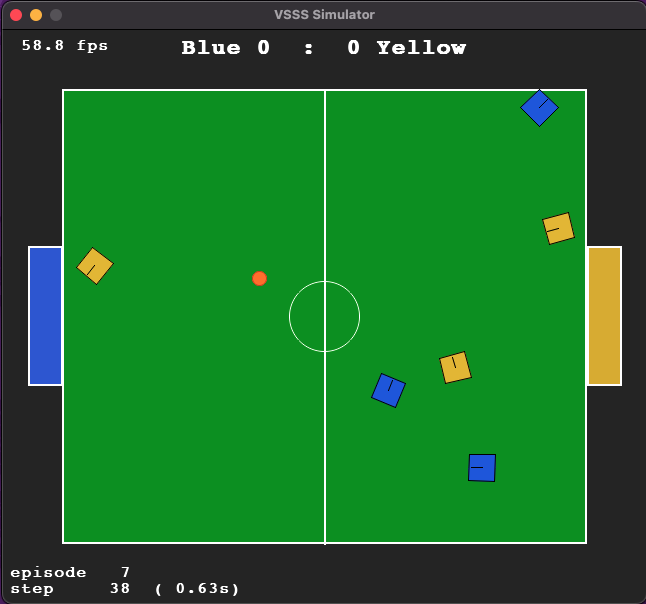
\includegraphics[width=0.8\textwidth]{Cap5/pygame_window.png}
    \caption{Pygame window showing a 3v3 match with the oriented-bounding-box robot shapes, direction indicators, and HUD.}
    \label{fig:pygame_window}
\end{figure}

% ------------------------------------------------------------------
\subsection{Prioritized-Level-Replay Sampler}
% ------------------------------------------------------------------

The third preliminary result concerns the prioritized-level-replay sampler,
which in TG-1 is established at the level of design and supporting
infrastructure rather than full evaluation.

The mechanism that the sampler will hook into is already in place.  Episode
initialization is controlled by a pluggable \texttt{InitMode}, currently
offering a standard kickoff formation (with small random jitter) and a fully
randomized mode that places robots and the ball uniformly across the field.
Both backends implement randomized reset, and the JAX implementation is
\texttt{vmap}-ready, so a batch of distinct initial configurations can be
generated on device in a single call.  Critically, the initialization interface
was designed to accommodate a future selector mode, in which an external model
supplies the placement distribution rather than a fixed rule — this is exactly
the insertion point the \gls{plr} sampler requires.

For TG-1, the contract the sampler must satisfy is defined: it receives
per-scenario statistics from completed rollouts, updates a priority for each
stored scenario from the magnitude of the value-prediction error, and returns a
new batch of initial states biased toward high-priority scenarios while
retaining enough exploration to avoid collapsing onto a narrow set.  The TG-1
deliverable is the demonstration that this contract is compatible with the
batched simulator interface — that scenarios can be stored, scored, and
resampled without breaking vectorization.  Quantitative sample-efficiency
results, in particular learning curves against uniform initialization, are
deferred to TG-2.

% ------------------------------------------------------------------
\subsection{Early Training Validation}
\label{sec:early_training}
% ------------------------------------------------------------------

A final preliminary result is an end-to-end training smoke test confirming that
the \gls{ppo} loop runs correctly on the new simulator.  Using the batched
environment through the SB3 adapter, a Stage-1 configuration (the controlled
team alone, against stationary opponents) was trained with the shaped reward
described in Chapter~4: the sparse $\pm 1$ goal signal augmented by a small
dense term proportional to the ball's forward progress, with the shaping
coefficient set so that its total episodic contribution cannot exceed a single
goal event.  Training runs are tracked with MLflow, logging per-generation mean,
minimum, and maximum reward together with episode length.
Here, one generation denotes one complete episode rollout in each parallel
environment; for these runs, with 256 environments and a 300-step episode cap,
one generation equals $256 \times 300 = 76{,}800$ environment transitions.

The purpose of these early training experiments is not to produce a competitive
policy but to confirm that rollout collection, advantage estimation, optimization,
and checkpointing operate together correctly on the new infrastructure.
Table~\ref{tab:smoke_config} lists every setting that differs from the
simulator defaults or that is shared across both runs; the physics contract
(Table~\ref{tab:physics_design}, Chapter~4) and observation layout
(Table~\ref{tab:obs}) apply unchanged unless noted.
Both runs were executed on a MacBook with an Apple M4 Pro chip
(\texttt{scripts/smoke.py}, batched JAX backend via \texttt{VSSVecEnv}).
Any learning curve reported at this stage should be read as a functional
validation rather than a performance result.

\begin{table}[ht]
    \centering
    \caption{TG-1 smoke-test configuration
    (\texttt{scripts/smoke.py}).  Rows marked ``default'' use
    \texttt{vsss\_sim.config} or SB3 defaults unless overridden on the CLI.}
    \label{tab:smoke_config}
    \small
    \begin{tabular}{p{0.36\linewidth}p{0.22\linewidth}p{0.34\linewidth}}
        \toprule
        \textbf{Parameter} & \textbf{Value} & \textbf{Source} \\
        \midrule
        \multicolumn{3}{l}{\textit{Environment (both runs)}} \\
        Parallel environments     & $256$ & \texttt{--num-envs} \\
        Physics backend           & JAX (batched) & \texttt{VSSVecEnv} \\
        Controlled team           & Blue ($6$ actions) & \texttt{VSSEnv} \\
        Opponent policy           & Stationary & \texttt{opponent\_policy} \\
        Episode cap               & $300$ steps ($5$\,s) & \texttt{--max-episode-steps} \\
        Default episode cap       & $1200$ steps ($20$\,s) & \texttt{MAX\_EPISODE\_STEPS} (not used) \\
        Control frequency         & $60$\,Hz, $4$ sub-steps & \texttt{FPS}, \texttt{SUB\_STEPS} \\
        Reward                    & Eq.~\eqref{eq:reward}, $\beta=0.10$ & \texttt{BALL\_FORWARD\_REWARD\_COEF} \\
        Observation               & $\mathbb{R}^{46}$ (Table~\ref{tab:obs}) & default \\
        \midrule
        \multicolumn{3}{l}{\textit{PPO / SB3 (both runs)}} \\
        Algorithm / policy        & PPO, \texttt{MlpPolicy} & \texttt{PARAMS} \\
        Learning rate             & $3\times 10^{-4}$ & \texttt{PARAMS} \\
        Rollout length per env    & $300$ & \texttt{--n-steps} auto-aligned to episode cap \\
        PPO device                & CPU & \texttt{device="cpu"} in script \\
        \midrule
        \multicolumn{3}{l}{\textit{Run A (Figure~\ref{fig:plot_random})}} \\
        Initialization            & \texttt{InitMode.RANDOM} & \texttt{--init-mode random} \\
        Generations               & $900$ & \texttt{--generations 900} \\
        \midrule
        \multicolumn{3}{l}{\textit{Run B (Figure~\ref{fig:plot_kickoff})}} \\
        Initialization            & \texttt{InitMode.KICKOFF} & \texttt{--init-mode kickoff} (default) \\
        Generations               & $123$ & \texttt{--generations 123} \\
        \bottomrule
    \end{tabular}
\end{table}

Two initialization modes were compared.  In the first run, robots and the ball
were placed at uniformly random positions across the field at the start of each
episode (\texttt{InitMode.RANDOM}).  The per-generation mean reward over 900
generations is shown in Figure~\ref{fig:plot_random}.  Despite running for
nearly an order of magnitude more generations than the kickoff run, the policy
failed to make consistent progress: reward remains in the range $10^{-2}$
throughout training, with high variance and no discernible upward trend.  This
result is consistent with the known difficulty of random initialization in sparse
goal-scoring environments — the agent rarely encounters ball-near-goal
configurations from which meaningful reward can be obtained, so the gradient
signal is too weak to drive reliable improvement.

\begin{figure}[ht]
    \centering
    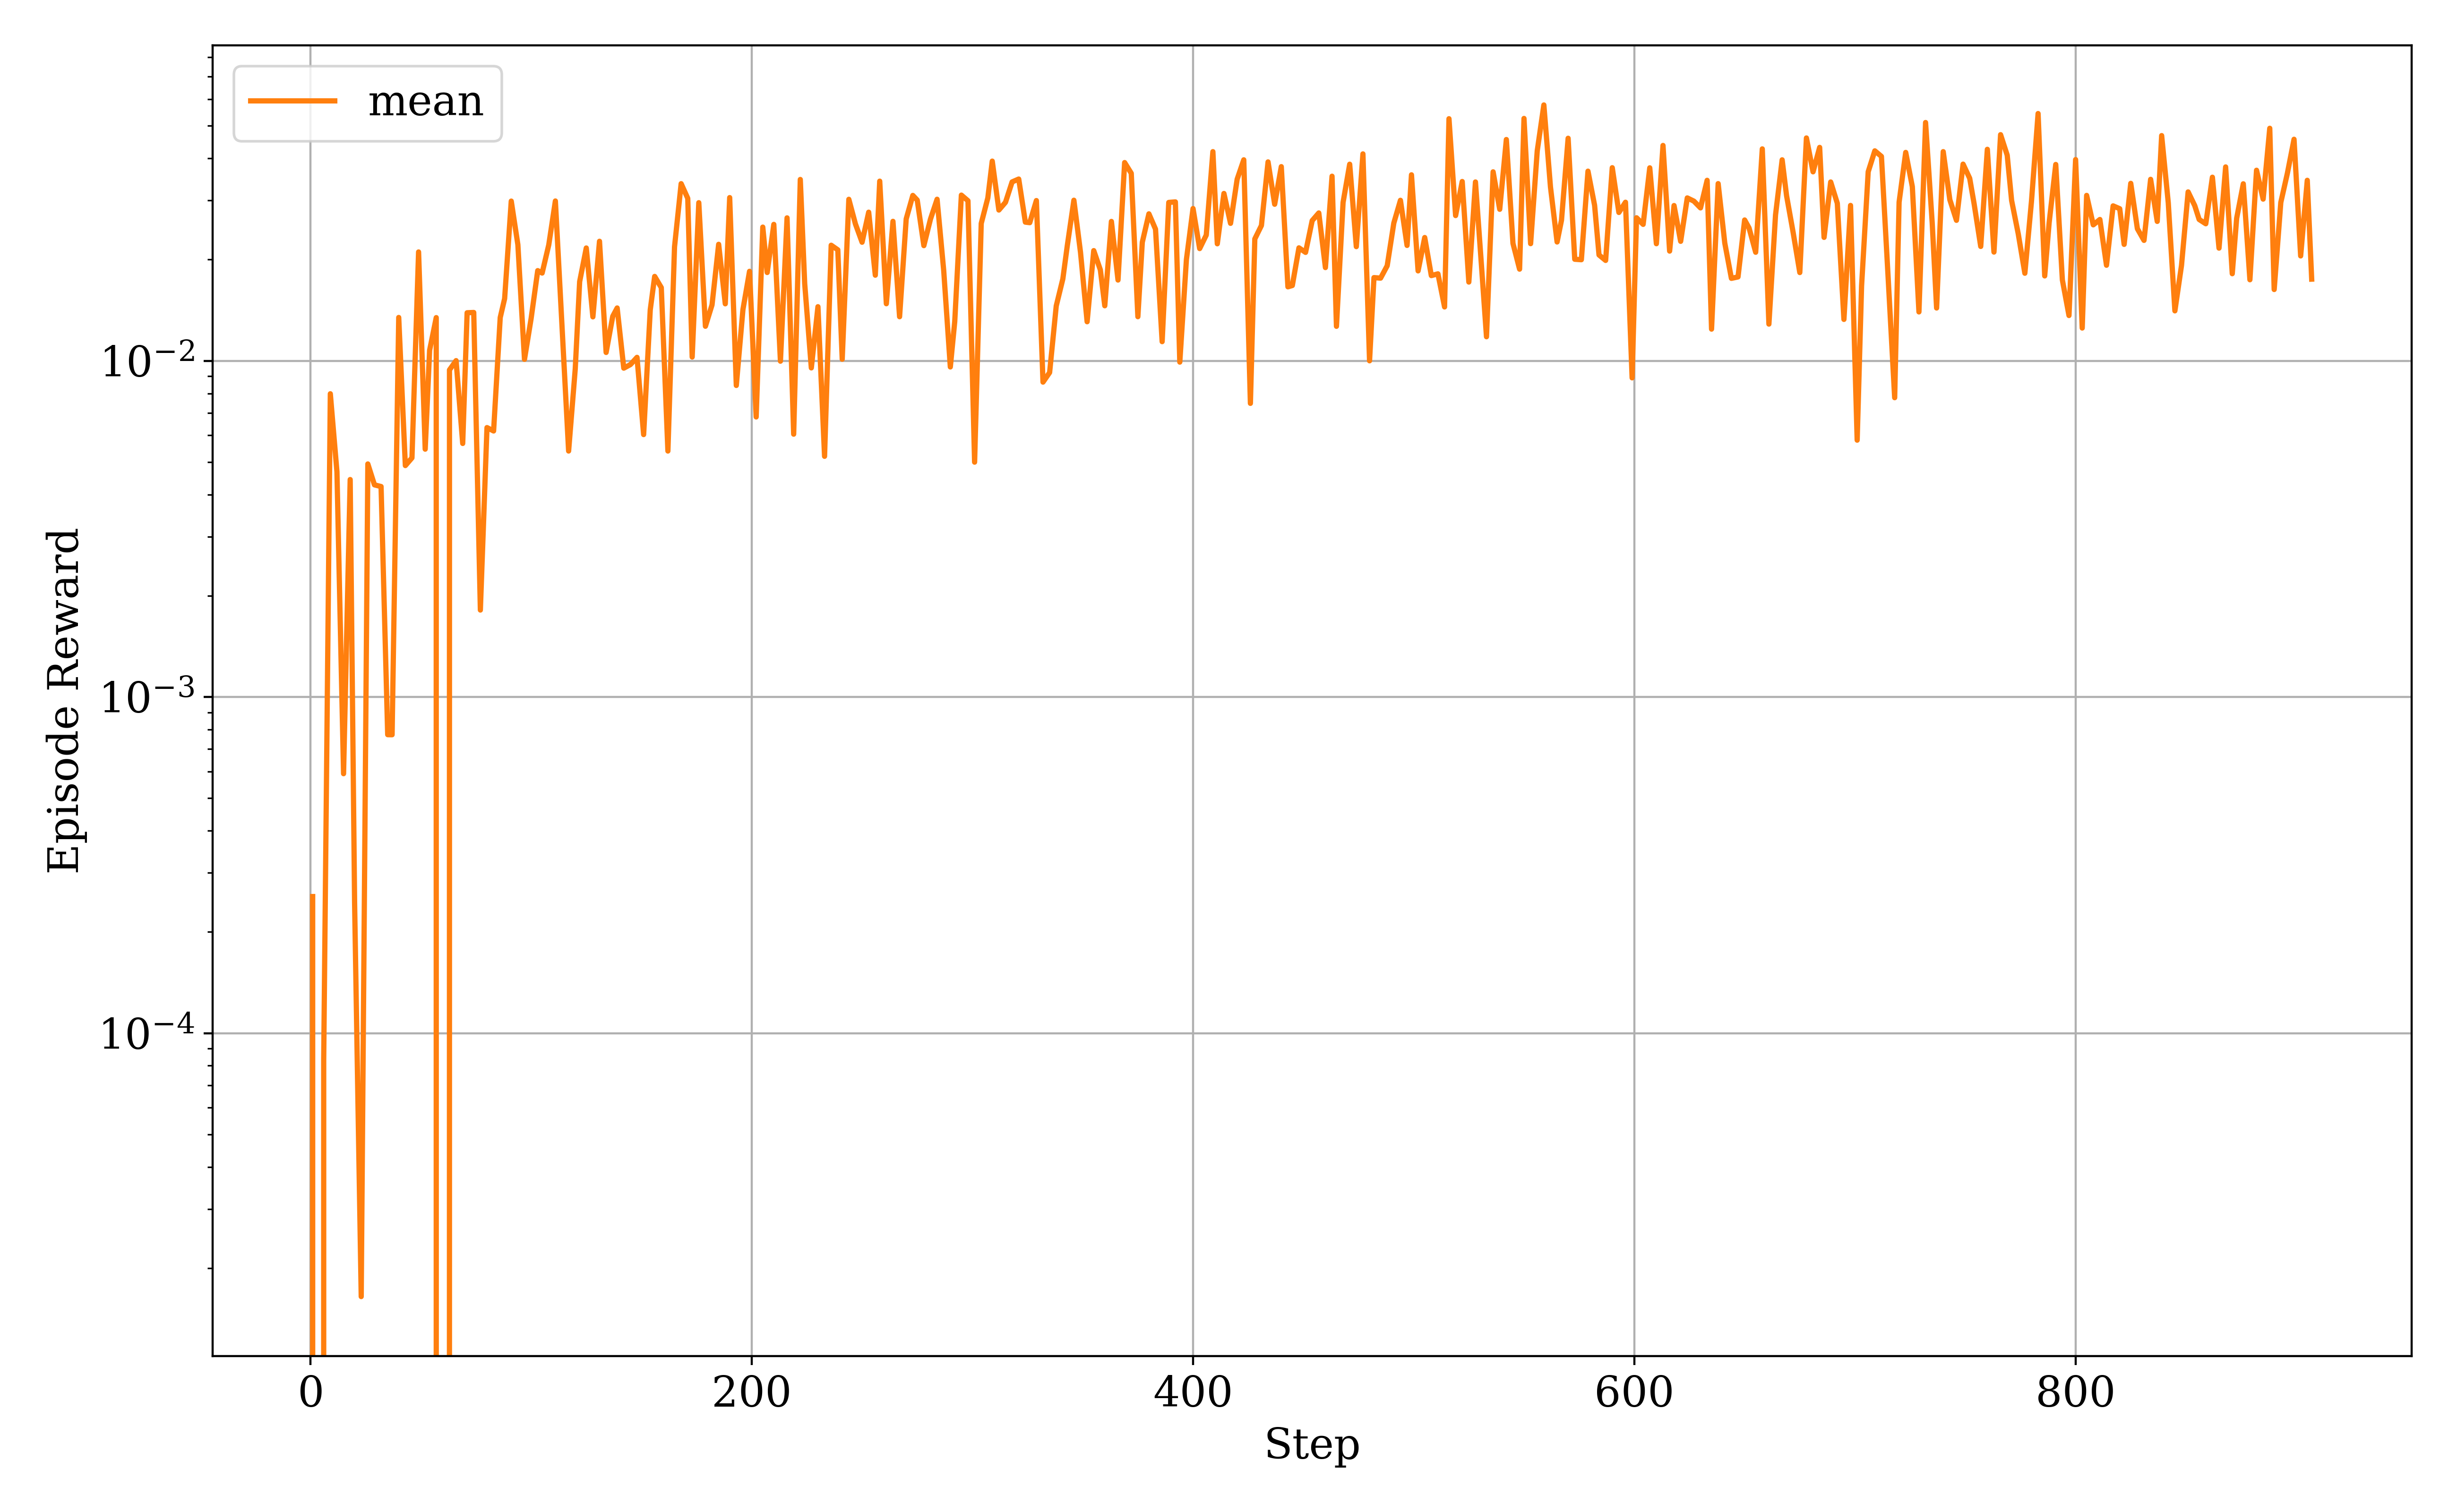
\includegraphics[width=0.85\textwidth]{Cap5/plot_random.png}
    \caption{Per-generation mean episode reward (log scale) for Run~A in
    Table~\ref{tab:smoke_config} (\texttt{InitMode.RANDOM}, 900 generations).
    The policy exhibits no
    consistent upward trend, confirming that flat random initialization provides
    insufficient learning signal in the sparse goal-scoring setting.}
    \label{fig:plot_random}
\end{figure}

In the second run, episodes began from the standard kickoff formation with small
random jitter (\texttt{InitMode.KICKOFF}), which places the ball at the centre
and the robots near their starting positions.  The per-generation mean and
minimum reward over 123 generations are shown in
Figure~\ref{fig:plot_kickoff}.  Here the policy improves rapidly: mean reward
is near zero for the first 50 generations and then rises steeply, reaching
approximately 2.0 by generation 120 — a value corresponding to consistent
multi-goal episodes.  The minimum reward tracks near zero throughout, indicating
that some environments within the batch fail to score while the mean is already
high, which is expected early in training when exploration varies widely across
parallel instances.

\begin{figure}[ht]
    \centering
    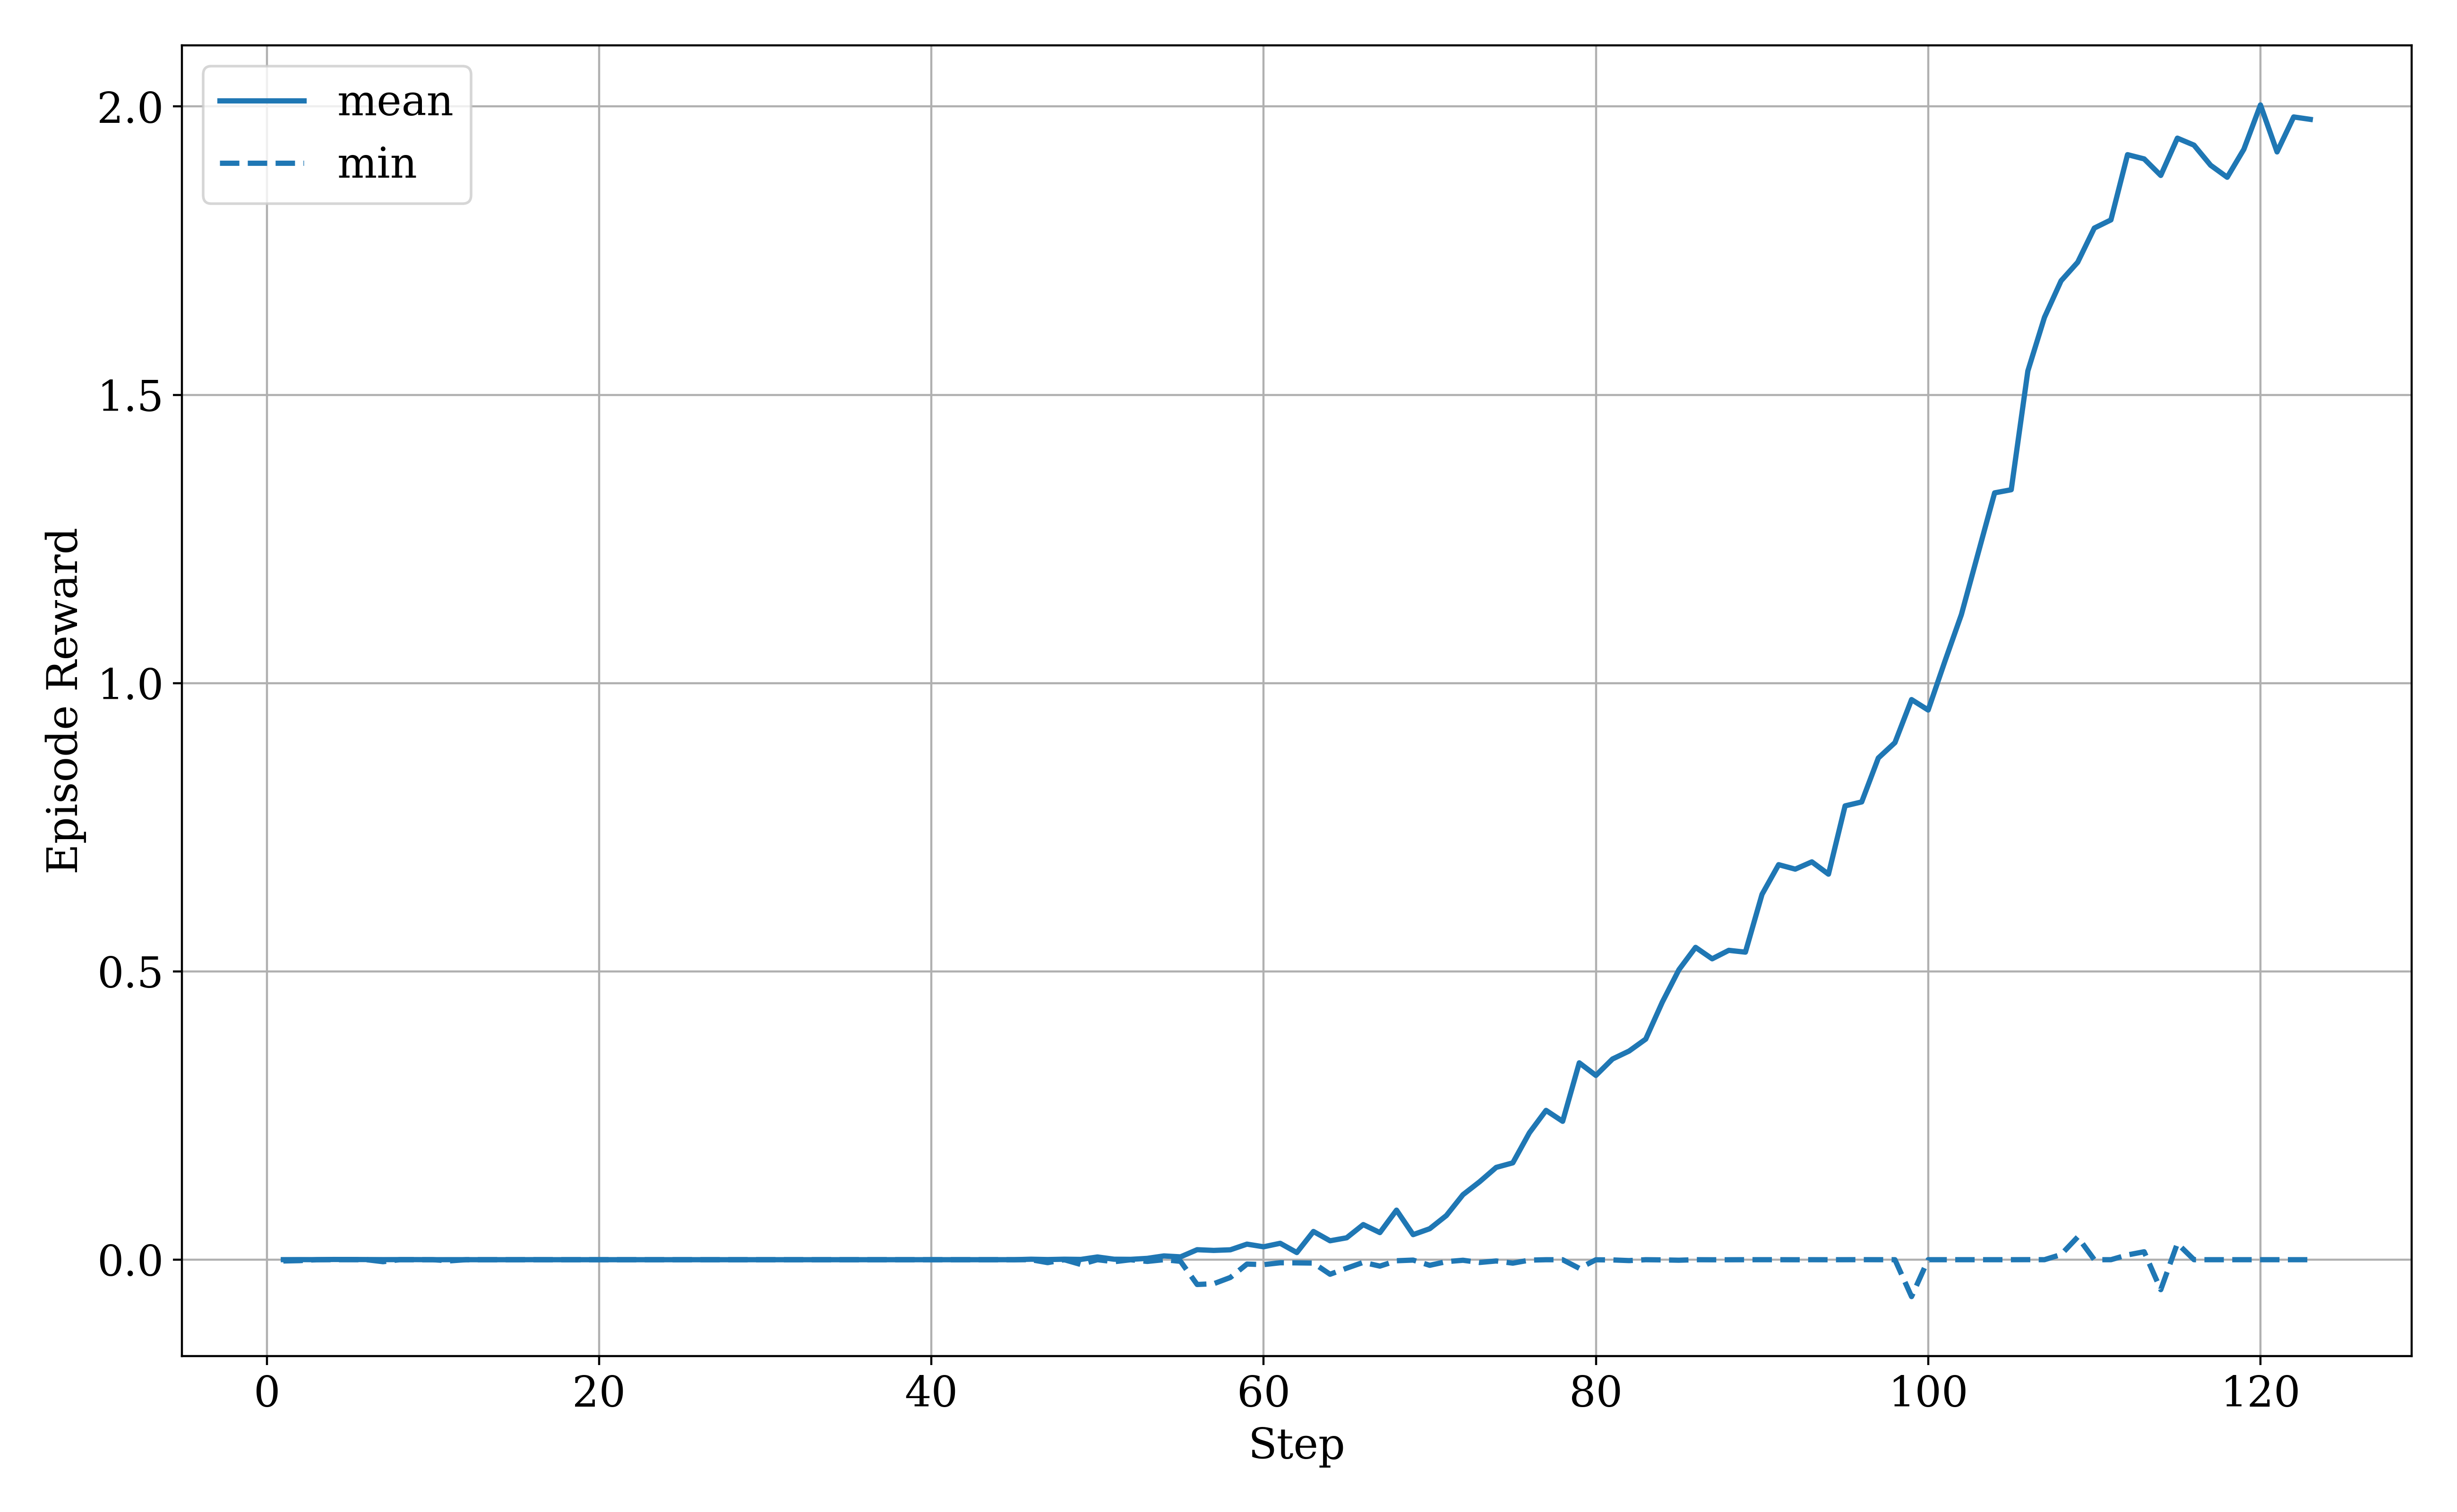
\includegraphics[width=0.85\textwidth]{Cap5/plot_kickoff.png}
    \caption{Per-generation mean and minimum episode reward for Run~B in
    Table~\ref{tab:smoke_config} (\texttt{InitMode.KICKOFF}, 123 generations).
    The policy converges rapidly
    once learning begins around generation 60, validating that the end-to-end
    training loop operates correctly under structured initialization.}
    \label{fig:plot_kickoff}
\end{figure}

Taken together, the two runs validate the training infrastructure and
simultaneously motivate the prioritized-level-replay curriculum planned for
TG-2.  Kickoff initialization is sufficient to confirm that the \gls{ppo} loop
works, but it does not cover the diversity of game states the policy must handle.
Random initialization covers that diversity but provides too sparse a signal to
drive learning.  The \gls{plr} sampler is designed precisely to interpolate
between these extremes: adaptively steering the distribution of initial states
toward configurations where the current policy's value-prediction error is
largest, thereby ensuring both sufficient difficulty and sufficient density of
learning signal throughout training.

% ==================================================================
\section{Future Planned Results}
\label{sec:future_planned_results}
% ==================================================================

The infrastructure validated above is the foundation for the experiments
planned for TG-2.  This section states what those experiments are and what each
is intended to show.

\subsection{Closing the throughput gap with a JAX-native learner.}
The throughput measurements identified two ceilings: the Gymnasium boundary and
the CPU-bound PyTorch updates of SB3.  Both stem from the learner living outside
the accelerator.  The planned remedy is a fully JAX-resident training path, in
which the policy, the rollout collection, and the gradient updates all execute
on device alongside the simulator, removing the per-step host transfers
entirely.  The target is to bring end-to-end \gls{ppo} throughput close to the
raw batched-kernel ceiling — on the order of $9 \times 10^{5}$ steps per second
on the RTX~3060, against the present $\sim 10^{4}$ of the SB3 path.  The expected
result is a before/after throughput comparison of the full training loop, not
merely the simulator in isolation.

\subsection{Prioritized-level-replay sample efficiency.}
With the sampler integrated, the central evaluation is whether prioritizing
high-learning-potential scenarios improves sample efficiency relative to uniform
initialization.  The planned result is a set of learning curves (reward and goal
rate versus environment steps) comparing the \gls{plr} sampler against a uniform
baseline under identical compute budgets, accompanied by qualitative inspection
of which scenarios the sampler prioritizes over the course of training.

\subsection{Two-stage curriculum and self-play.}
The opponents are currently stationary.  TG-2 will introduce the second
curriculum stage, replacing them with self-play opponents drawn from a history
of past policies, and will evaluate the effect of the opponent-sampling scheme
on the robustness of the learned team.  The planned result is a comparison of
policies trained with and without the curriculum, and with different
opponent-sampling strategies.

\subsection{Symmetry exploitation.}
TG-2 will quantify the benefit of the permutation- and reflection-symmetry
mechanisms described in Chapter~4, through an ablation comparing training with
and without symmetry-aware parameter sharing and data augmentation.

\subsection{Evaluation against the classical strategy.}
Finally, the trained team will be evaluated against the ITAndroids classical
strategy stack, reporting win rate, goal difference, and qualitative behavioral
analysis — the measure of whether a learned 3v3 team policy is competitive with
the hand-engineered baseline.  Sim-to-real considerations (domain randomization,
noise injection) frame this evaluation as a step toward eventual deployment, the
longer-term goal beyond TG-2.

\chapter{Conclusion}
\section{Summary}

This TG-1 report delivers the contributions stated in
Section~\ref{sec:contributions}: an accelerated simulator and a centralized
joint-policy training baseline for 3v3 IEEE Very Small Size Soccer.  The
throughput measurements show that the batched JAX design substantially exceeds
the conventional CPU-based, socket-mediated architecture, while the training
runs confirm that the simulator can support an end-to-end \gls{ppo} loop rather
than only fast isolated stepping.

The training results also clarify the next methodological step.  Kickoff
initialization produces reliable learning, whereas uniform random
initialization fails to provide enough useful signal.  This contrast motivates
the prioritized-level-replay sampler as the TG-2 mechanism for choosing
informative initial situations.

\section{Roadmap to TG-2}

The concrete TG-2 experiments are detailed in
Section~\ref{sec:future_planned_results}: closing the end-to-end throughput gap
with a JAX-native learner, evaluating the
prioritized-level-replay sampler, extending the curriculum to self-play,
measuring symmetry-aware improvements, and comparing the learned team against
the ITAndroids classical strategy stack.  Together, these experiments will
determine whether the simulator and training infrastructure built in TG-1 can
produce a robust, competitive 3v3 \gls{vsss} team policy and define the next
steps toward eventual deployment.

Table~\ref{tab:gantt} shows the planned schedule for the TG-2 development period.

\definecolor{ganttblue}{RGB}{70,130,180}
\begin{table}[ht]
    \centering
    \caption{TG-2 planned schedule (Jun--Nov 2026).  Shaded cells indicate the
    months in which each task is active.}
    \label{tab:gantt}
    \setlength{\tabcolsep}{6pt}
    \begin{tabular}{l|cccccc}
        \toprule
        \textbf{Task} & \textbf{Jun} & \textbf{Jul} & \textbf{Aug} & \textbf{Sep} & \textbf{Oct} & \textbf{Nov} \\
        \midrule
        Finish TG-1               & \cellcolor{ganttblue!70} &                          &                          &                          &                          &                          \\
        JAX-native learner        & \cellcolor{ganttblue!70} & \cellcolor{ganttblue!70} &                          &                          &                          &                          \\
        PLR sampler               &                          & \cellcolor{ganttblue!70} &                          &                          &                          &                          \\
        Symmetry exploitation     &                          & \cellcolor{ganttblue!70} & \cellcolor{ganttblue!70} &                          &                          &                          \\
        Self-play curriculum      &                          & \cellcolor{ganttblue!70} & \cellcolor{ganttblue!70} &                          &                          &                          \\
        Evaluation \& comparison  &                          &                          & \cellcolor{ganttblue!70} & \cellcolor{ganttblue!70} & \cellcolor{ganttblue!70} & \cellcolor{ganttblue!70} \\
        TG-2 writing              &                          &                          &                          &                          & \cellcolor{ganttblue!70} & \cellcolor{ganttblue!70} \\
        \bottomrule
    \end{tabular}
\end{table}

% REFERENCIAS BIBLIOGRAFICAS
\renewcommand\bibname{\itareferencesnamebabel} %renomear título do capítulo referências
\printbibliography

% Apendices e anexos podem ser habilitados quando houver material complementar.
% \appendix
% \chapter{Supplementary Material}
% \section{Disclaimer: Use of AI}

\color{red}
This thesis was written using the help of AI, mainly for reviewing the text,
and for formatting and academic tone matching.

Also, some of the development of the Simulator code and scripting was leveraged by the use of AI tools.

\color{black}

%
% \annex
% \chapter{External Material}
% \input{AneA/anexoA}

% Glossario
%\itaglossary
%\printglossary

% Folha de Registro do Documento
% Valores dos campos do formulario
\FRDitadata{29 May 2026}
\FRDitadocnro{DCTA/ITA/DM-018/2026} %(o número de registro você solicita a biblioteca)
\FRDitaorgaointerno{Instituto Tecnológico de Aeronáutica -- ITA}
%Exemplo no caso de pós-graduação: Instituto Tecnol{\'o}gico de Aeron{\'a}utica -- ITA
\FRDitapalavrasautor{Reinforcement learning; Multi-agent systems; Very Small Size Soccer; GPU simulation}
\FRDitapalavrasresult{Reinforcement learning; Multi-agent systems; Robotics; Simulation}
%Exemplo no caso de graduação (TG):
%\FRDitapalavraapresentacao{Trabalho de Graduação, ITA, São José dos Campos, 2026. \NumPenultimaPagina\ páginas.}
%Exemplo no caso de pós-graduação (msc, dsc):
\FRDitapalavraapresentacao{Bachelor's Thesis, ITA, São José dos Campos, 2026. Advisor: Prof.~Dr. Marcos Máximo.}
\FRDitaresumo{Este trabalho aborda o treinamento por aprendizado por reforço em larga escala no futebol de robôs IEEE Very Small Size Soccer em partidas 3v3 por meio de duas contribuições: um simulador em GPU baseado em JAX, capaz de executar milhares de partidas em paralelo, e uma pipeline de treinamento PPO para uma política centralizada de equipe. O throughput de treinamento PPO de ponta a ponta alcança aproximadamente $49{.}000$--$58{.}000$ passos por segundo (com 256 e 65{.}536 ambientes paralelos em um Apple M4~Pro e uma NVIDIA RTX~3060, respectivamente), em comparação com 63--378 passos por segundo nas configurações de treinamento anteriores do ITAndroids baseadas em ODE — um ganho de duas a três ordens de grandeza. Parte dessa vantagem decorre da arquitetura em lote residente no acelerador; parte reflete um modelo físico 2D deliberadamente mais simples, uma troca discutida no texto. Essa pipeline serve como a linha de base do TG-1 para as extensões de seleção de amostras e de aprendizado multiagente descentralizado planejadas para o TG-2.

Os resultados de treinamento confirmam que a infraestrutura suporta aprendizado de política confiável e revelam que a estratégia de inicialização é um fator crítico: a inicialização por formação de kickoff produz aprendizado rápido, enquanto a inicialização aleatória uniforme não fornece sinal de gradiente suficiente. Essa observação motiva diretamente o amostrador baseado em prioritized level replay, que será implementado e avaliado no TG-2, juntamente com a arquitetura descentralizada por robô e o currículo completo com autojogo.}
%  Primeiro Parametro: Nacional ou Internacional -- N/I
%  Segundo parametro: Ostensivo, Reservado, Confidencial ou Secreto -- O/R/C/S
\FRDitaOpcoes{N}{O}
% Cria o formulario
\itaFRD

\end{document}
% Fim do Documento. O massacre acabou!!! :-)
